\documentclass[sigconf]{acmart}
% \documentclass{...}
%\documentclass[11pt, letterpaper]{article}
\usepackage[margin=1in]{geometry}

% \documentclass[11pt, letterpaper]{article}
% 
% % ----- margins -----
% 
% \topmargin -1.5cm         % read Lamport p.163
% \oddsidemargin -0.04cm    % read Lamport p.163
% \evensidemargin -0.04cm   % same as oddsidemargin but for left-hand pages
% 
% % ----- texts -----
% 
% \textwidth 16.59cm
% \textheight 21.94cm
% 
% % ----- indendts and spacing -----
% 
% \parskip 0pt            	% spacing between paragraphs
% %\renewcommand{\baselinestretch}{1.5}	% uncomment for 1.5 spacing
% 
% \parindent 7mm		      % leading space for paragraphs between lines
% 
% % ----- page # -----
% 
% %\pagestyle{empty}         % uncomment if don't want page numbers





%=== use the these packages if they are not already in use ===
%\usepackage{amsfonts}
%\usepackage{amsmath}
%\usepackage{amssymb}
\usepackage{amsthm}
\usepackage{bbm} 
%\usepackage{cite}
\usepackage{color}
%\usepackage{euscript}
\usepackage{graphicx}
\usepackage{mathrsfs} 
%\usepackage{microtype}
% \usepackage[normalem]{ulem}
% \usepackage{wrapfig}
%=============================================================

%===== control =====
\allowdisplaybreaks

%===== fonts =====
\def\ttt{\texttt}
\def\tsc{\textsc}

%===== spacing =====

\def\extraspacing{\vspace{3mm} \noindent}
\def\figcapup{\vspace{-1mm}}
\def\figcapdown{\vspace{-0mm}}
\def\hgap{\textrm{\hspace{1mm}}}
\def\thmvgap{\vspace{0mm}}
\def\vgap{\vspace{1mm}}


%===== tabbing =====

\def\tab{\hspace{3mm}}
\def\tabpos{\hspace{4mm} \= \hspace{4mm} \= \hspace{4mm} \= \hspace{4mm} \= \hspace{4mm} \= \hspace{4mm} \= \hspace{4mm} \= \hspace{4mm} \= \hspace{4mm} \= \hspace{4mm} \= \hspace{4mm} \= \hspace{4mm} \= \hspace{4mm} \= \hspace{4mm} %\= 
%\= \hspace{4mm} \= \hspace{4mm} \= \hspace{4mm} \= \hspace{4mm} \= \hspace{4mm} \= \hspace{4mm}
\kill}
\newcommand{\mytab}[1]{\begin{tabbing}\tabpos #1\end{tabbing}}

%===== blocks =====

%%%%%%%%%%%%%%%%%%%%%%%%%%%%%%%%
% THEOREMS
%%%%%%%%%%%%%%%%%%%%%%%%%%%%%%%%
% \theoremstyle{plain}
% \newtheorem{theorem}{Theorem}[section]
% \newtheorem{proposition}[theorem]{Proposition}
% \newtheorem{lemma}[theorem]{Lemma}
% \newtheorem{corollary}[theorem]{Corollary}
% \theoremstyle{definition}
% \newtheorem{definition}[theorem]{Definition}
% \newtheorem{assumption}[theorem]{Assumption}
% \theoremstyle{remark}
% \newtheorem{remark}[theorem]{Remark}

% \newtheorem{theorem}{Theorem}
% \newtheorem{lemma}[theorem]{Lemma}
% \newtheorem{corollary}[theorem]{Corollary}
% \newtheorem{proposition}{Proposition}
% \newtheorem{definition}{Definition}
% \newtheorem{problem}{Problem}

\newcommand{\boxminipg}[2]{\begin{center}\fbox{\begin{minipage}{#1}#2\end{minipage}}\end{center}}
\newcommand{\minipg}[2]{\begin{center}\begin{minipage}{#1}#2\end{minipage}\end{center}}
\newcommand{\myitems}[1]{\begin{itemize} #1 \end{itemize}}
\newcommand{\myenums}[1]{\begin{enumerate} #1 \end{enumerate}}
\newcommand{\myfig}[1]{\begin{figure}\centering #1\end{figure}}
\newcommand{\myfigg}[2]{\begin{figure}\centering #1 \figcapup \caption{#2} \figcapdown \end{figure}}
\newcommand{\myfigstar}[2]{\begin{figure*}\centering #1 \figcapup \caption{#2} \figcapdown \end{figure*}}

%===== math macros =====

\newcommand{\bm}[1]{\textrm{\boldmath${#1}$}}
\newcommand{\mb}[1]{\mathbf{#1}}
% \newcommand{\smat}[2]{\left[\begin{tabular}{#1}#2\end{tabular}\right]}
% \newcommand{\bmat}[2]{\left|\begin{tabular}{#1}#2\end{tabular}\right|}
\newcommand{\bmat}[1]{\begin{bmatrix}#1\end{bmatrix}}
\newcommand{\vmat}[1]{\begin{vmatrix}#1\end{vmatrix}}
\newcommand{\myeqn}[1]{\begin{eqnarray}#1\end{eqnarray}}
\newcommand{\myset}[1]{\{#1\}}
\newcommand{\set}[1]{\{#1\}}

\newcommand{\explain}[1]{(\textrm{#1})}
%\newcommand{\bracket}[1]{\left(#1\right)}
%\newcommand{\dbar}[1]{\Vert#1\Vert}
%\newcommand{\one}[1]{\mathbbm{1}\{#1\}}

%\def\bm{\boldmath}
%\def\defeq{\stackrel{\textrm{\tiny{def}}}{=}}
\def\mit{\mathit}
\def\defeq{:=}
\def\eps{\epsilon}
\def\fr{\frac}
\def\-{\mbox{-}}
\def\ol{\overline}
\def\real{\mathbb{R}}
\def\intdom{\mathbb{N}}

\def\tO{\tilde{O}}
\def\tOmega{\tilde{\Omega}}

\def\lc{\left \lceil}
\def\lf{\left \lfloor}
\def\rc{\right \rceil}
\def\rf{\right \rfloor}
\newcommand{\ceil}[1]{\lceil #1 \rceil}
\newcommand{\floor}[1]{\lfloor #1 \rfloor}

\def\nn{\nonumber}

\def\Pr{\mathbf{Pr}}
%\def\expt{\mathbf{E}}
\def\var{\mathbf{Var}}

\def\dcl{\{\!\!\{}
\def\dcr{\}\!\!\}}
\def\bigdcl{\Big\{\!\!\Big\{}
\def\bigdcr{\Big\}\!\!\Big\}}
\def\bigmid{\textrm{ $\Big|$ }}


\DeclareMathOperator*{\argmin}{arg\,min}
\DeclareMathOperator*{\argmax}{arg\,max}
\DeclareMathOperator*{\polylog}{polylog}
\DeclareMathOperator*{\poly}{poly}
\DeclareMathOperator*\expt{\mathbf{E}}
%\DeclareMathOperator*\Pr{\mathbf{Pr}}

%===== misc =====

\def\done{\qed \vspace{2mm}}	% end of proof
\def\tbc{\hspace*{\fill} $\textrm{{\em (to be continued)}}\blacktriangle$ \vspace{2mm}}
%\def\done{\hspace*{\fill} $\Box$}	% end of proof
\allowdisplaybreaks
%===== coloring =====

\newcommand{\red}[1]{\textcolor{red}{#1}}
\newcommand{\blue}[1]{\textcolor{blue}{\bf #1}}
\newcommand{\purple}[1]{\textcolor{purple}{\bf #1}}
\newcommand{\todo}[1]{\textcolor{red}{\bf [TO DO: #1]}}


%=================================
%Yufei's stuff
%\usepackage{amsmath}
\usepackage{balance}
%\usepackage{times}
\usepackage{microtype}

\def\vgap{\vspace{1mm}}
\def\extraspacing{\vspace{2mm} \noindent}
\def\figcapup{\vspace{-0mm}}
\def\figcapdown{\vspace{-0mm}}

\def\A{\mathcal{A}}
\def\B{\mathcal{B}}
\def\C{\mathcal{C}}
\def\E{\mathcal{E}}
\def\G{\mathcal{G}}
\def\I{\mathcal{I}}
\def\J{\mathcal{J}}
\def\II{\mathscr{I}}
\def\L{\mathcal{L}}
\def\P{\mathcal{P}}
\def\Q{\mathcal{Q}}
\def\R{\mathcal{R}}
\def\T{\mathcal{T}}
\def\U{\mathcal{U}}
\def\V{\mathcal{V}}
\def\X{\mathcal{X}}
\def\XX{\mathscr{X}}
\def\Y{\mathcal{Y}}
\def\YY{\mathscr{Y}}
\def\Z{\mathcal{Z}}

\def\xleft{\mathrm{left}}
\def\xright{\mathrm{right}}
\def\ybot{\mathrm{bot}}
\def\ytop{\mathrm{top}}
\def\maxtop{\mathrm{maxtop}}
\def\minleft{\mathrm{minleft}}
\def\gleft{\mathrm{left\text{-}guard}}
\def\gbot{\mathrm{bot\text{-}guard}}
\def\cross{\mathrm{cross}}
\def\dcross{\mathrm{d\text{-}cross}}
\def\contained{\mathrm{contained}}
\def\cat{\mathrm{cat1}}
\def\catt{\mathrm{cat2}}
\def\out{\mathrm{OUT}}



\allowdisplaybreaks
%=================================

%====== from acm ======
\acmDOI{}
\acmISBN{}

\acmConference[]{...}{...}{...}
\acmYear{...}
\copyrightyear{}
\acmArticle{}
\acmPrice{}
%======================



\begin{document}
%\begin{sloppy}
    
\title{Optimal (Multiway) Spatial Joins}

% \author{}
% \affiliation{
% 	\institution{Chinese University of Hong Kong}
% 	\city{Hong Kong}
% 	\country{China}}	

\author{}


\begin{abstract}
    In a {\em spatial join}, we are given a constant number $k \geq 2$ of sets containing axis-parallel rectangles in a 2D space, denoted as $R_1, R_2, ..., R_k$. The objective is to report all $k$-tuples $(r_1, r_2, ..., r_k) \in R_1 \times R_2 \times ... \times R_k$ where the rectangles $r_1, r_2, ..., r_k$ have a non-empty intersection, i.e., $r_1 \cap r_2 \cap ... \cap r_k \neq \emptyset$. The problem holds significant importance in spatial databases and has been extensively studied in the database community. In this paper, we show how to settle the problem in $O(n \log n + \out)$ time --- regardless of the constant $k$ --- where $n = \sum_{i=1}^k |R_i|$ and $\out$ is the result size (i.e., the total number of $k$-tuples reported). The runtime  is asymptotically optimal in the class of comparison-based algorithms, to which our solution belongs. Our result significantly improves the state of the art, which is an algorithm with running time $O(n \log^{2k} n + \out)$.
\end{abstract}

\maketitle 

\section{Introduction} \label{sec:intro}

This paper studies the {\em spatial join} (SJ) problem formulated as follows. Let $k \ge 2$ be a constant integer. In the {\em $k$-SJ} problem, the input comprises $k$ sets --- denoted as $R_1, R_2, ..., R_k$ --- of axis-parallel rectangles\footnote{A rectangle is {\em axis-parallel} if it has the form $r = [x_1, x_2] \times [y_1, y_2]$.} in $\real^2$. The goal is to find all $k$-tuples $(r_1, r_2, ..., r_k)$ where
\myitems{
    \item $r_i \in R_i$ for each $i \in [1, k]$; and
    \item $r_1 \cap r_2 \cap ... \cap r_k \neq \emptyset$, namely, the $k$ rectangles $r_1, r_2, ..., r_k$ have a non-empty intersection.
}
We represent the set of $k$-tuples described above as $\J(R_1, R_2, ..., R_k)$, referred to as the {\em join result}. Set $n = \sum_{i=1}^k |R_i|$, i.e., the input size, and $\out = |\J(R_1, R_2, ..., R_k)|$, i.e., the output size.

\vgap

SJ is a fundamental operation in spatial databases (SDB), which manage geometric entities such as land parcels, service areas, habitat zones, commercial districts, administrative boundaries, etc. The operation plays a crucial role in implementing the {\em filter-refinement mechanism}, which is the dominant approach for computing overlay information in an SDB. To explain this mechanism, first note that a geometric entity is typically modeled as a polygon. Determining whether two entities overlap amounts to deciding if two polygons intersect, which can be exceedingly expensive when the polygons have complex boundaries. To mitigate the issue, an SDB stores, for each polygon $\gamma$, its {\em minimum bounding rectangle} (MBR) defined as the smallest axis-parallel rectangle enclosing $\gamma$; this way, each set $\Gamma$ of geometric entities spawns a set $R$ of MBRs. Consider $k$ sets of geometric entities $\Gamma_1, \Gamma_2, ..., \Gamma_k$, and the corresponding sets of MBRs $R_1, R_2, ..., R_k$. To compute overlays from $\Gamma_1, \Gamma_2, ..., \Gamma_k$, filter-refinement first executes (i) a ``filter step'', which performs an SJ to obtain $\J(R_1, R_2, ..., R_k)$, and (ii) a ``refinement step'', which, for each $(r_1, r_2, ..., r_k) \in \J(R_1, R_2, ..., R_k)$, examines if $\gamma_1, \gamma_2, ..., \gamma_k$ indeed have a non-empty intersection, where $\gamma_i$ ($i \in [1, k]$) is the entity in $\Gamma_i$ whose MBR is $r_i$.

%Two polygons $P_1$ and $P_2$ can overlap with each other only if their MBRs $r_1$ and $r_2$ intersect.

\extraspacing {\bf Math Conventions.} For any integer $x \ge 1$, we use $[x]$ to represent the set $\set{1, 2, ..., x}$. Given $k \ge 2$ sets $S_1, S_2, ..., S_k$ (of arbitrary elements), we often treat a $k$-tuple $\bm{t} = (e_1, e_2, .., e_k)$ in the cartesian product $S_1 \times S_2 \times ... \times S_k$ as a $k$-dimensional vector such that $\bm{t}[i] = e_i$ for each $i \in [k]$. Every mention of the word ``rectangle'' henceforth will refer to an axis-parallel rectangle. All logarithms have base 2 by default.

\subsection{Previous Results} \label{sec:intro:prev}

SJs have been extensively studied in the database-system community, leading to the development of numerous methods that, although lacking strong theoretical guarantees, exhibit good empirical performance in real-world applications. We refer interested readers to \cite{apr+00,bks93,gcn+13,js07,ks97,lr94,lr96,mp98,mp01,mp03,pd96,pmt99} as entry points into the literature.

\vgap

From the perspective of theory, SJs are best understood when $k = 2$, i.e., the {\em pairwise} scenario, where it is folklore that the problem can be solved in $O(n \log n + \out)$ time (e.g., by planesweep \cite{bcko08}). However, the problem becomes much more challenging for $k \ge 3$, known as the {\em multiway} scenario. All the solutions developed  before 2022 (see \cite{gcn+13,mp98,mp01,pmt99} and the references therein) suffer from a worst-case time complexity of $O(n^k)$, offering essentially no improvement over the naive method that enumerates the entire cartesian product $R_1 \times R_2 \times ... \times R_k$.

\vgap

Year 2022 witnessed two independent works \cite{ty22,kcko22} that, although not tackling $k$-SJ directly, imply provably fast $k$-SJ algorithms. Specifically, in \cite{ty22}, Tao and Yi studied several variants of ``interval intersection joins'' under updates. Most relevant to our context is the variant where the input includes, for each $i \in [k]$, a set $\I_i$ of 1D intervals in $\real$, and the join result comprises all $k$-tuples $(I_1,$ $I_2,$ $..., I_k) \in \I_1 \times \I_2 \times ... \times \I_k$ with $\bigcap_{i=1}^k I_i \neq \emptyset$. The objective is to design a data structure, which, given the insertion (resp., deletion) of an interval in one of the $k$ sets, can identify all the newly-appearing (resp., disappearing) $k$-tuples in the join result in $O((1+\Delta) \cdot \polylog n)$ time, where $n = \sum_{i=1}^k |\I_i|$ and $\Delta$ is the number of such $k$-tuples. Tao and Yi \cite{ty22} presented a structure of $O(n \polylog n)$ space achieving the purpose. Combining their structure with planesweep, one can obtain an algorithm for solving the $k$-SJ problem in $O((n + \out) \cdot \polylog n)$ time.

\vgap

In \cite{kcko22}, Khamis et al.\ investigated a type of joins that extends the conventional equi-join in two ways. First, each attribute value in a relation is an interval (rather than a real value); second, each equality predicate in equi-join is replaced with a ``non-empty intersection'' predicate on the attributes involved. The $k$-SJ problem can be converted to solving a join defined next under the framework of \cite{kcko22}. For each $i \in [k]$, define $R_i$ as a relation over two attributes $X$ and $Y$. For each tuple $\bm{t} \in R_i$, its values $\bm{t}(X)$ and $\bm{t}(Y)$ on the two attributes are both intervals (effectively defining a rectangle). The objective is to output all $k$-tuples $(\bm{t}_1, \bm{t}_2, ..., \bm{t}_k) \in R_1 \times R_2 \times ... \times R_k$ satisfying $\bigcap_{i=1}^k \bm{t}_i(X) \ne \emptyset$ and $\bigcap_{i=1}^k \bm{t}_i(Y) \ne \emptyset$. It is clear that there is one-one correspondence between the result of this join and that of k-SJ. Khamis et al.\ \cite{kcko22} developed an algorithm that can process the join  in $O(n \log^{2k} n + \out)$ time.

\vgap 

It is worth noting that $\Omega(n \log n)$ is a lower bound on the runtime of any comparison-based algorithm solving the $k$-SJ problem, even for $k = 2$. This can be established via a reduction from the {\em element distinctness} (ED) problem; see \cite{dl79}.

%where we are given $n$ real values $e_1, e_2, ..., e_n$ and need to decide whether there are distinct $i, j \in [n]$ satisfying $e_i = e_j$. The ED problem demands $\Omega(n \log n)$ comparisons to solve \cite{dl79}.

\begin{table} 
    \begin{tabular}{c|c|c|c} 
        $\bm{k}$ & {\bf method} & {\bf runtime} & {\bf remark} \\
        \hline\hline 
        2 & folklore & $O(n \log n + \out)$ & optimal \\ 
        \hline
        $\ge 3$ & before 2022 & $O(n^k)$ &  \\
        $\ge 3$ & \cite{ty22} & $O((n + \out) \cdot \polylog n)$ & \\
        $\ge 3$ & \cite{kcko22} & $O(n \log^{2k} n + \out)$ & \\
        \hline
        $\ge 3$ & ours & $O(n \log n + \out)$ & optimal
    \end{tabular}
    
    \vspace{3mm}
    \figcapup 
    \caption{Result comparison on $k$-SJ problem for a constant $k$}
    \label{tab:results-com}
    \figcapdown \vspace{-5mm}
\end{table}

\subsection{Our Results} \label{sec:intro:ours} 

In this paper, we solve the $k$-SJ problem with a comparison-based algorithm that runs in $O(n \log n + \out)$ time regardless of the constant $k$. The time complexity is asymptotically optimal.

\vgap 

In terms of techniques, our primary contribution is the revelation of a new property on the problem's mathematical structure. Fix any $k \ge 3$ and an {\em arbitrary} algorithm $\A$ for the $(k-1)$-SJ problem. For any $n \ge 1$, define function $F_{k-1}(n, \out)$ to return the worst-case running time of $\A$ on any instance of the $(k-1)$-SJ problem having input size at most $n$ and output size at most $\out$. Our core technical contribution is to establish:

\begin{theorem} \label{thm:main-recur}
    Equipped with the algorithm $\A$ as described above, the $k$-SJ problem can be solved in time
    \myeqn{
        O(k^3) \cdot \big( F_{k-1}(n, \out) + n \log n + k \cdot \out \big)
        %\nn
        \label{eqn:main:reccurrence}
    }
    where $n$ (resp., $\out$) is the input (resp., output) size of the problem.
%     time using $O(n + \out)$ space, plus the worst-case space of $\A$ on any $(k-1)$-SJ instance with input size $n$ and output size $\out$.
\end{theorem}

The theorem implies the existence of a recursive nature of $k$-SJ. Indeed, we will see that the $k$-SJ can be converted to $O(k^3)$ instances of the $(k-1)$-SJ problem --- all of which have input size at most $n$ and output size at most $\out$ --- plus an additional processing cost of $O(n \log n + \out)$. Furthermore, if $\A$ is comparison-based, so is the $k$-SJ algorithm that ensues. For 2-SJ, we can set $\A$ simply to the ``folklore algorithm'' mentioned in Section~\ref{sec:intro:prev}, which ensures $F_2(n, \out) = O(n \log n + \out)$. Combining this with \eqref{eqn:main:reccurrence} yields a recurrence that relates the time complexity of $k$-SJ to that of $(k-1)$-SJ. Solving the recurrence yields:

\begin{theorem} \label{thm:main-alg}
    For $k \ge 3$, we can settle $k$-SJ with a comparison-based algorithm in $O( c^k (k!)^3 \cdot (n \log n + k \cdot \out))$ time.
    %and $O(k \cdot n + \out)$ space, where $c > 1$ is a positive constant.
\end{theorem}


When $k = O(1)$, the time complexity becomes $O(n \log n$ $+ \out)$, as promised; the space consumption of our algorithm is $O(n + \out)$. Now that Theorem~\ref{thm:main-alg} offers a satisfactory $k$-SJ result for $k = O(1)$ in 2D space, it is natural to wonder whether the constraint on dimensionality 2 is necessary. Interestingly, the answer is ``yes'' as far as $k \ge 3$ is concerned, subject to the absence of breakthroughs on a classical problem in graph theory. Specifically, if the 3D version of the 3-SJ problem (which we will formally define in Appendix~\ref{app:lb-cond}) could be solved in $O(n \polylog n + \out)$ time, we would obtain an algorithm that detects the presence of a triangle (i.e., 3-clique) in a graph of $m$ edges in $O(m \polylog m)$ time, which would make a truly remarkable breakthrough because the state of the art needs $O(m^{1.41})$ time \cite{ayz97}. This reduction can be inferred from an argument in \cite{kcko22} used to prove a more generic result. We simplify the argument for 3D 3-SJ and present the full reduction in Appendix~\ref{app:lb-cond}.

\begin{figure}
    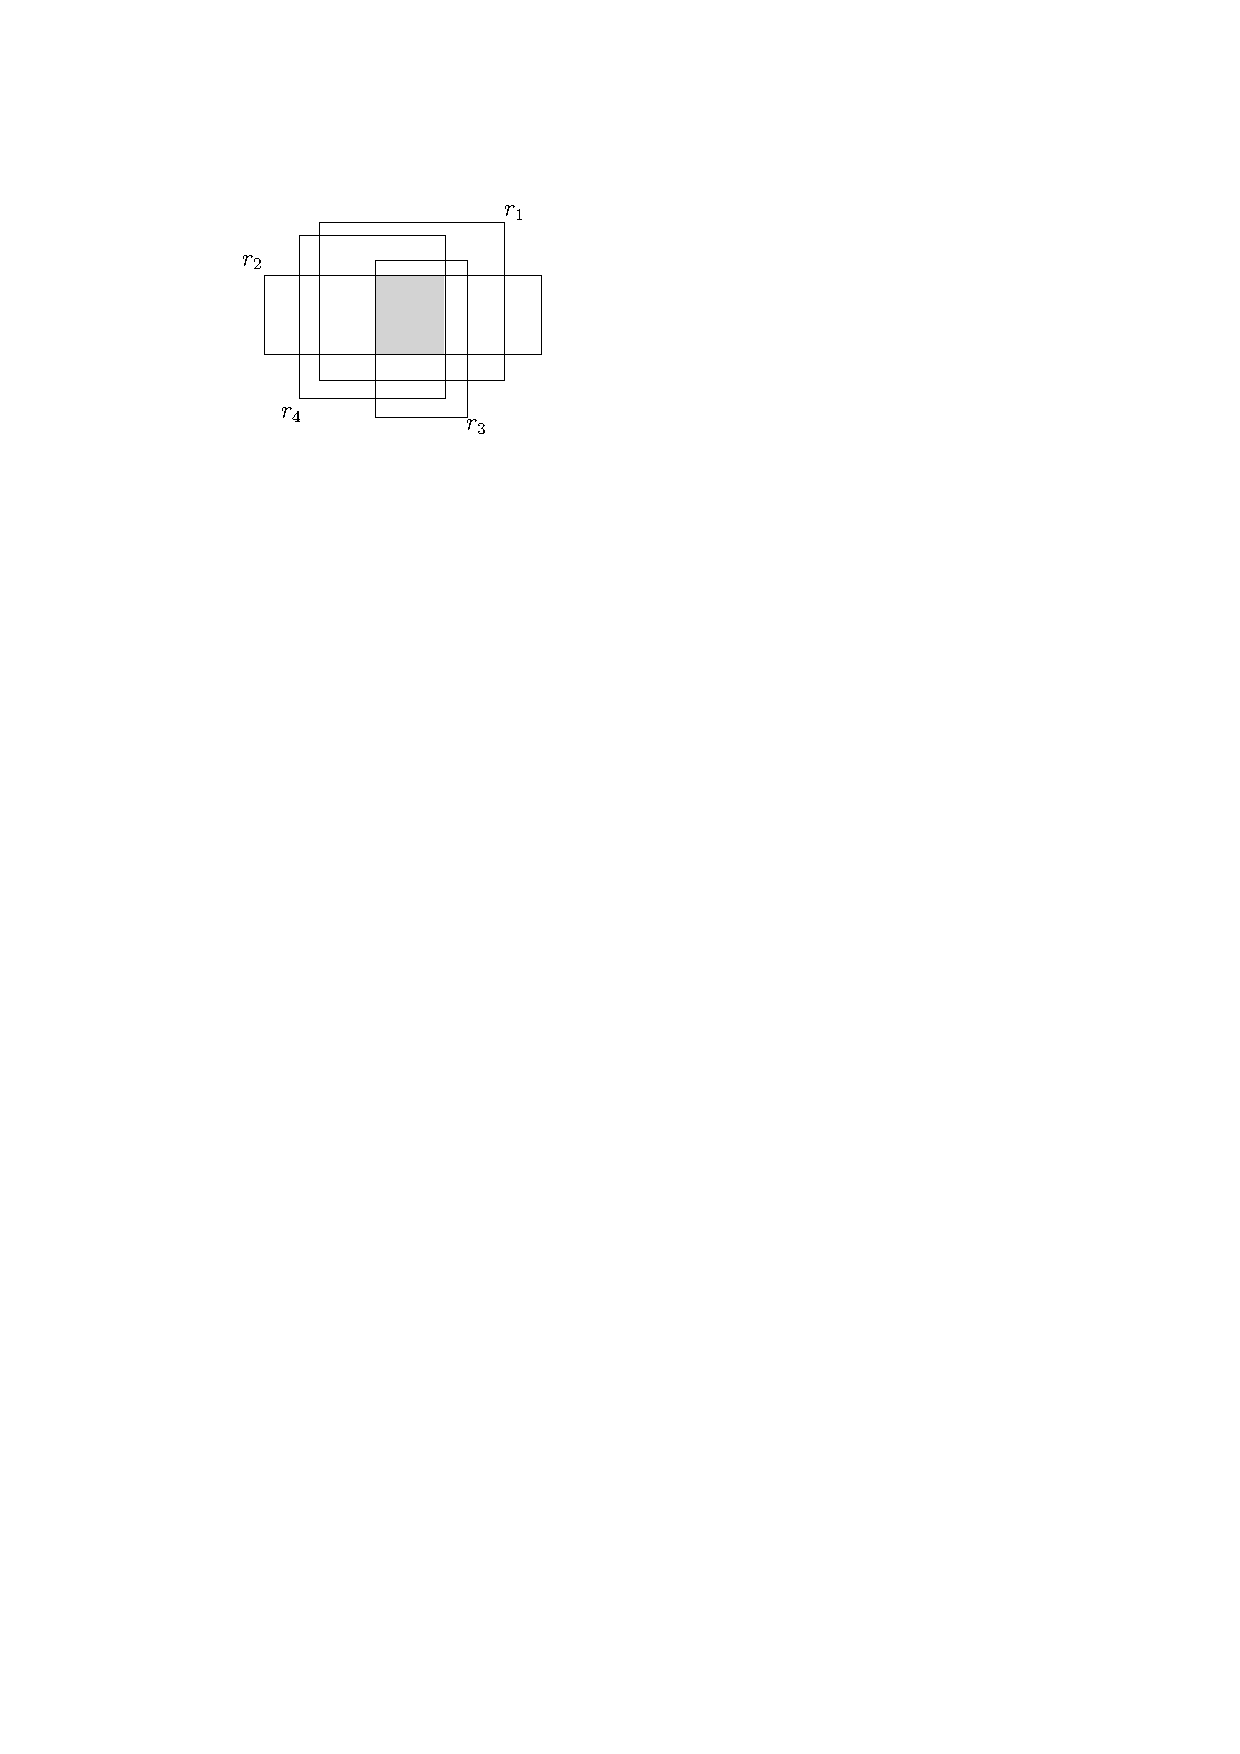
\includegraphics[height=27mm]{./artwork/guard}

    \figcapup
    \caption{Consider a 4-tuple $\bm{t} = \set{r_1, r_2, r_3, r_4}$. $B_\bm{t}$ is the rectangle in gray, $\gleft(\bm{t}) = r_3$ and $\gbot(\bm{t}) = r_2$.}
    \label{fig:guard}
    \figcapdown
\end{figure}


\begin{figure*}
    \begin{tabular}{ccccc}
        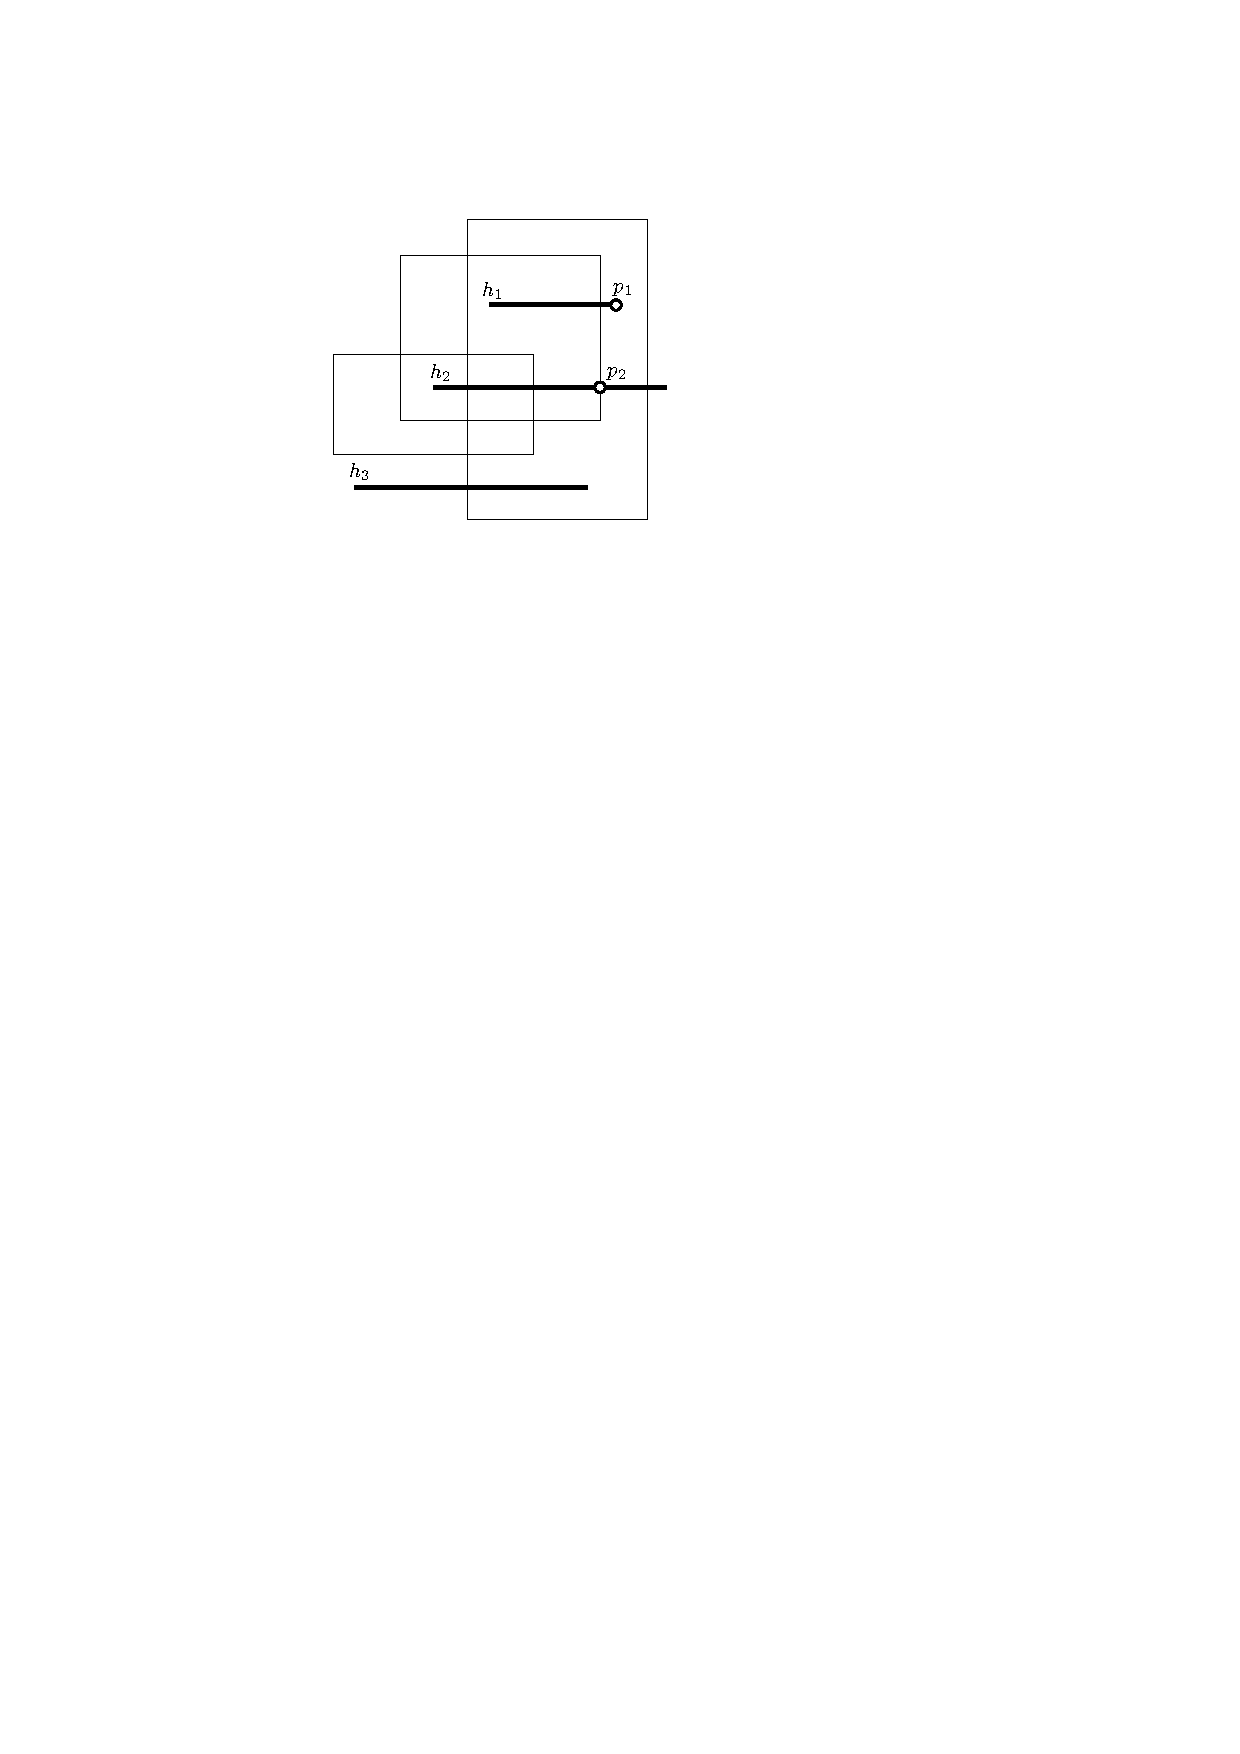
\includegraphics[height=30mm]{./artwork/prob-a} & 
        \hspace{3mm}
        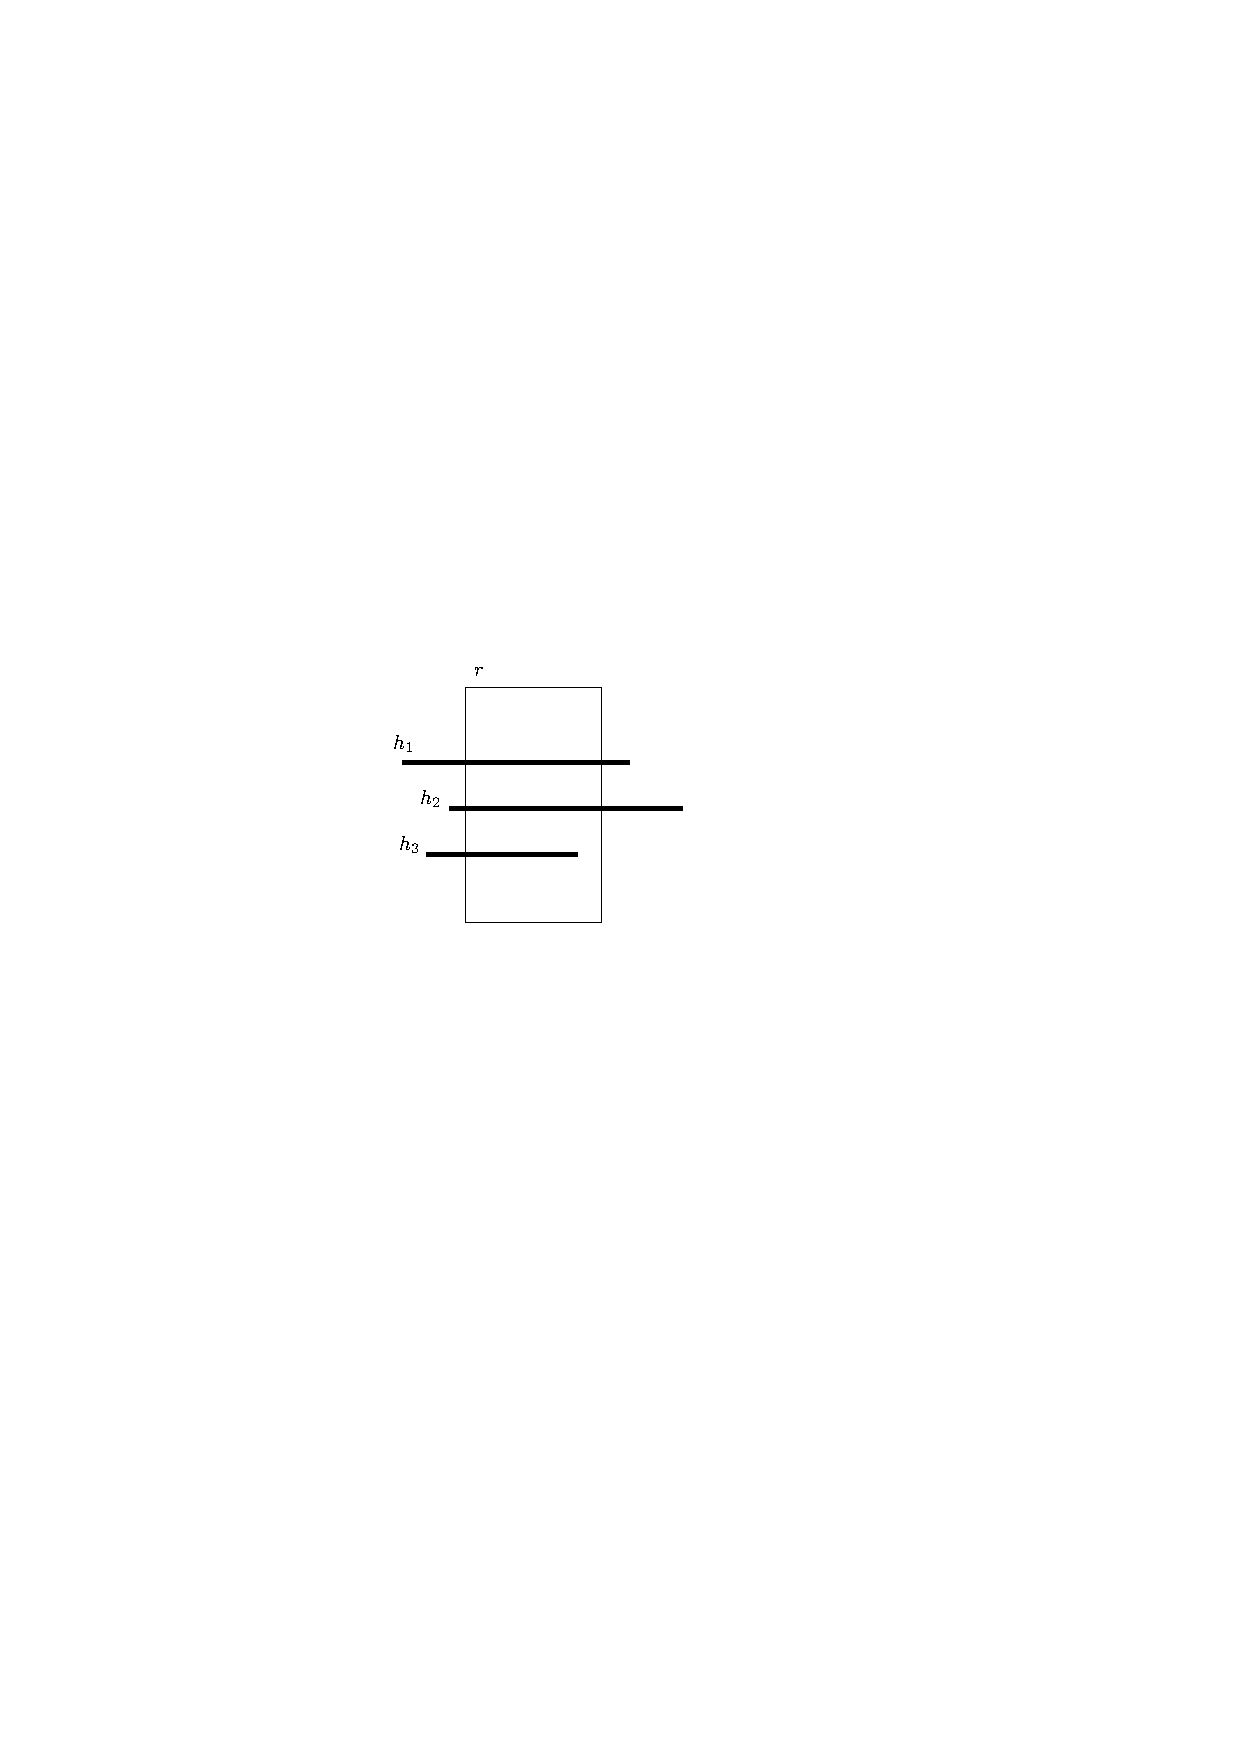
\includegraphics[height=27mm]{./artwork/prob-b} &
        \hspace{3mm}
        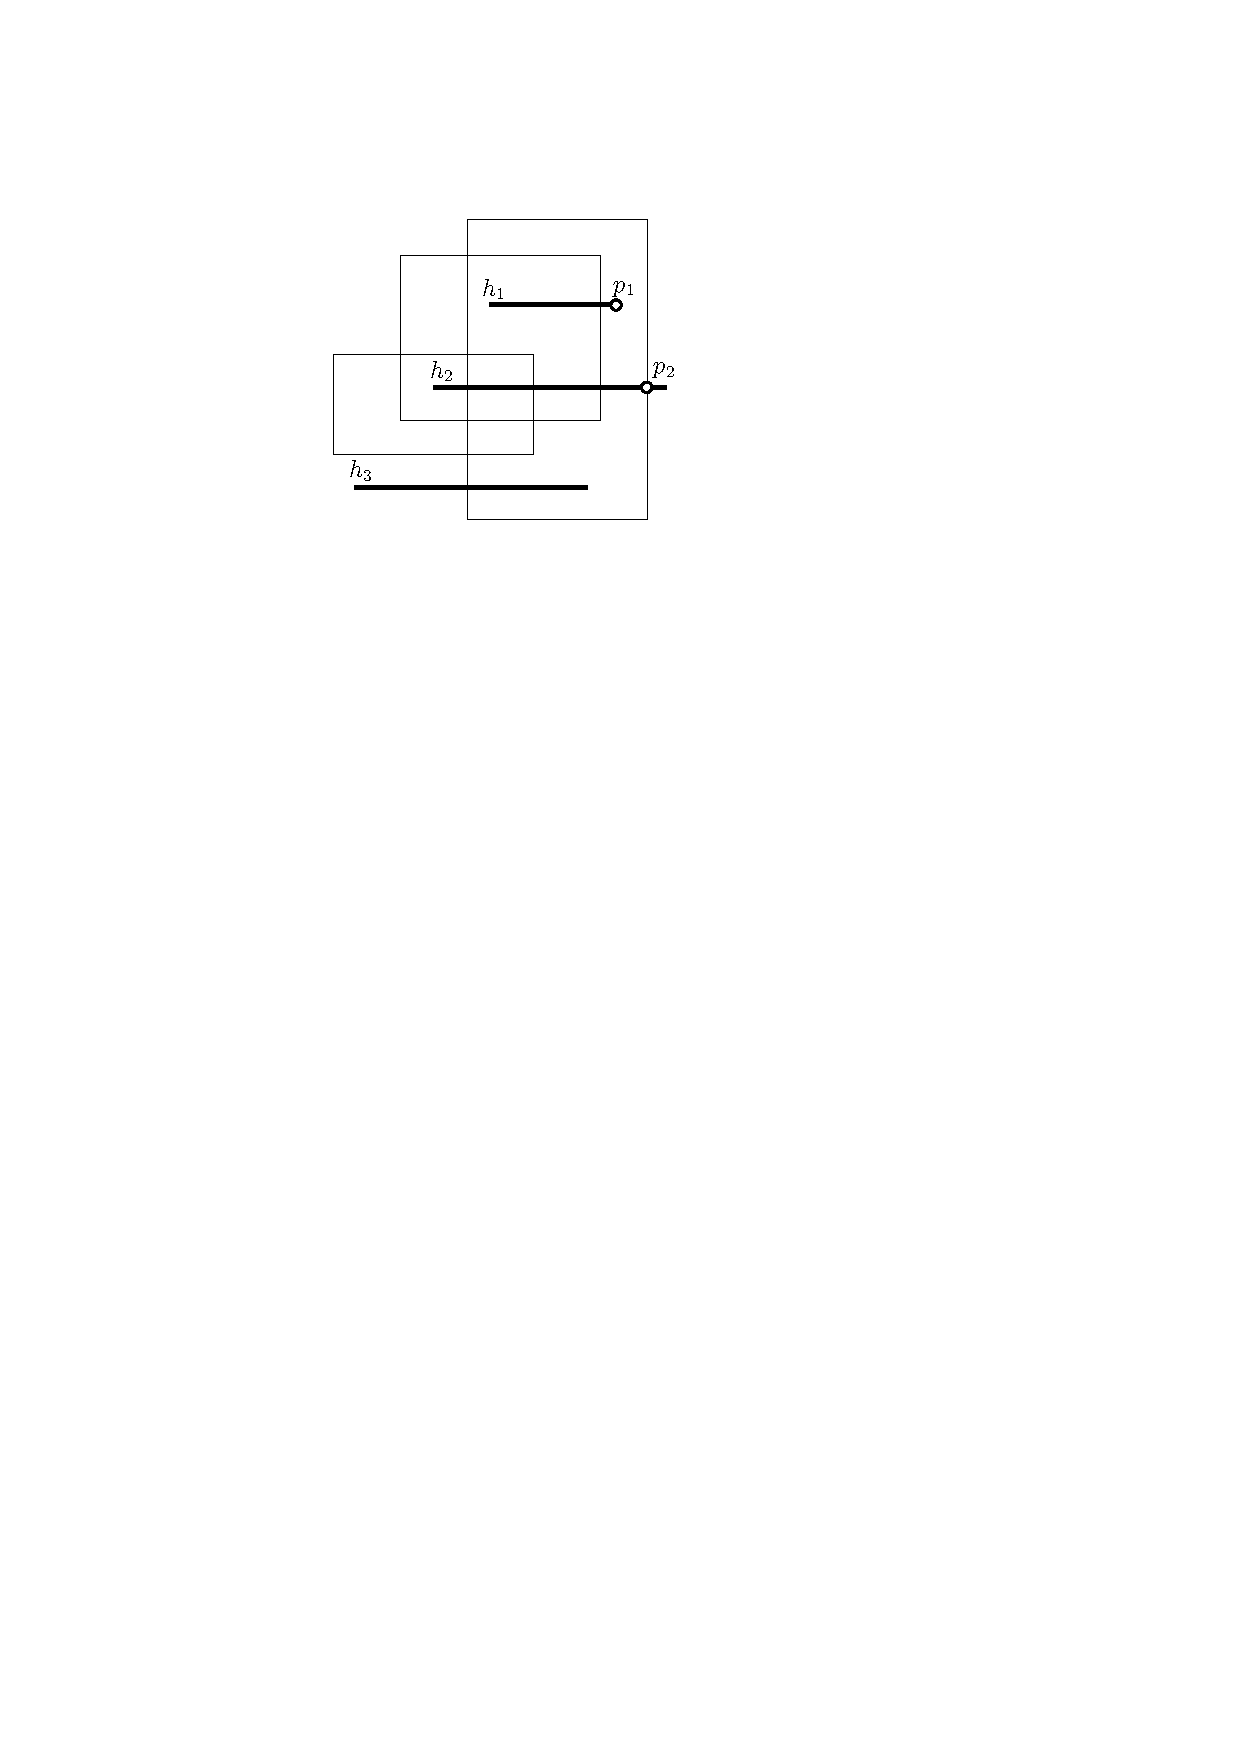
\includegraphics[height=30mm]{./artwork/prob-c} &
        \hspace{3mm}
        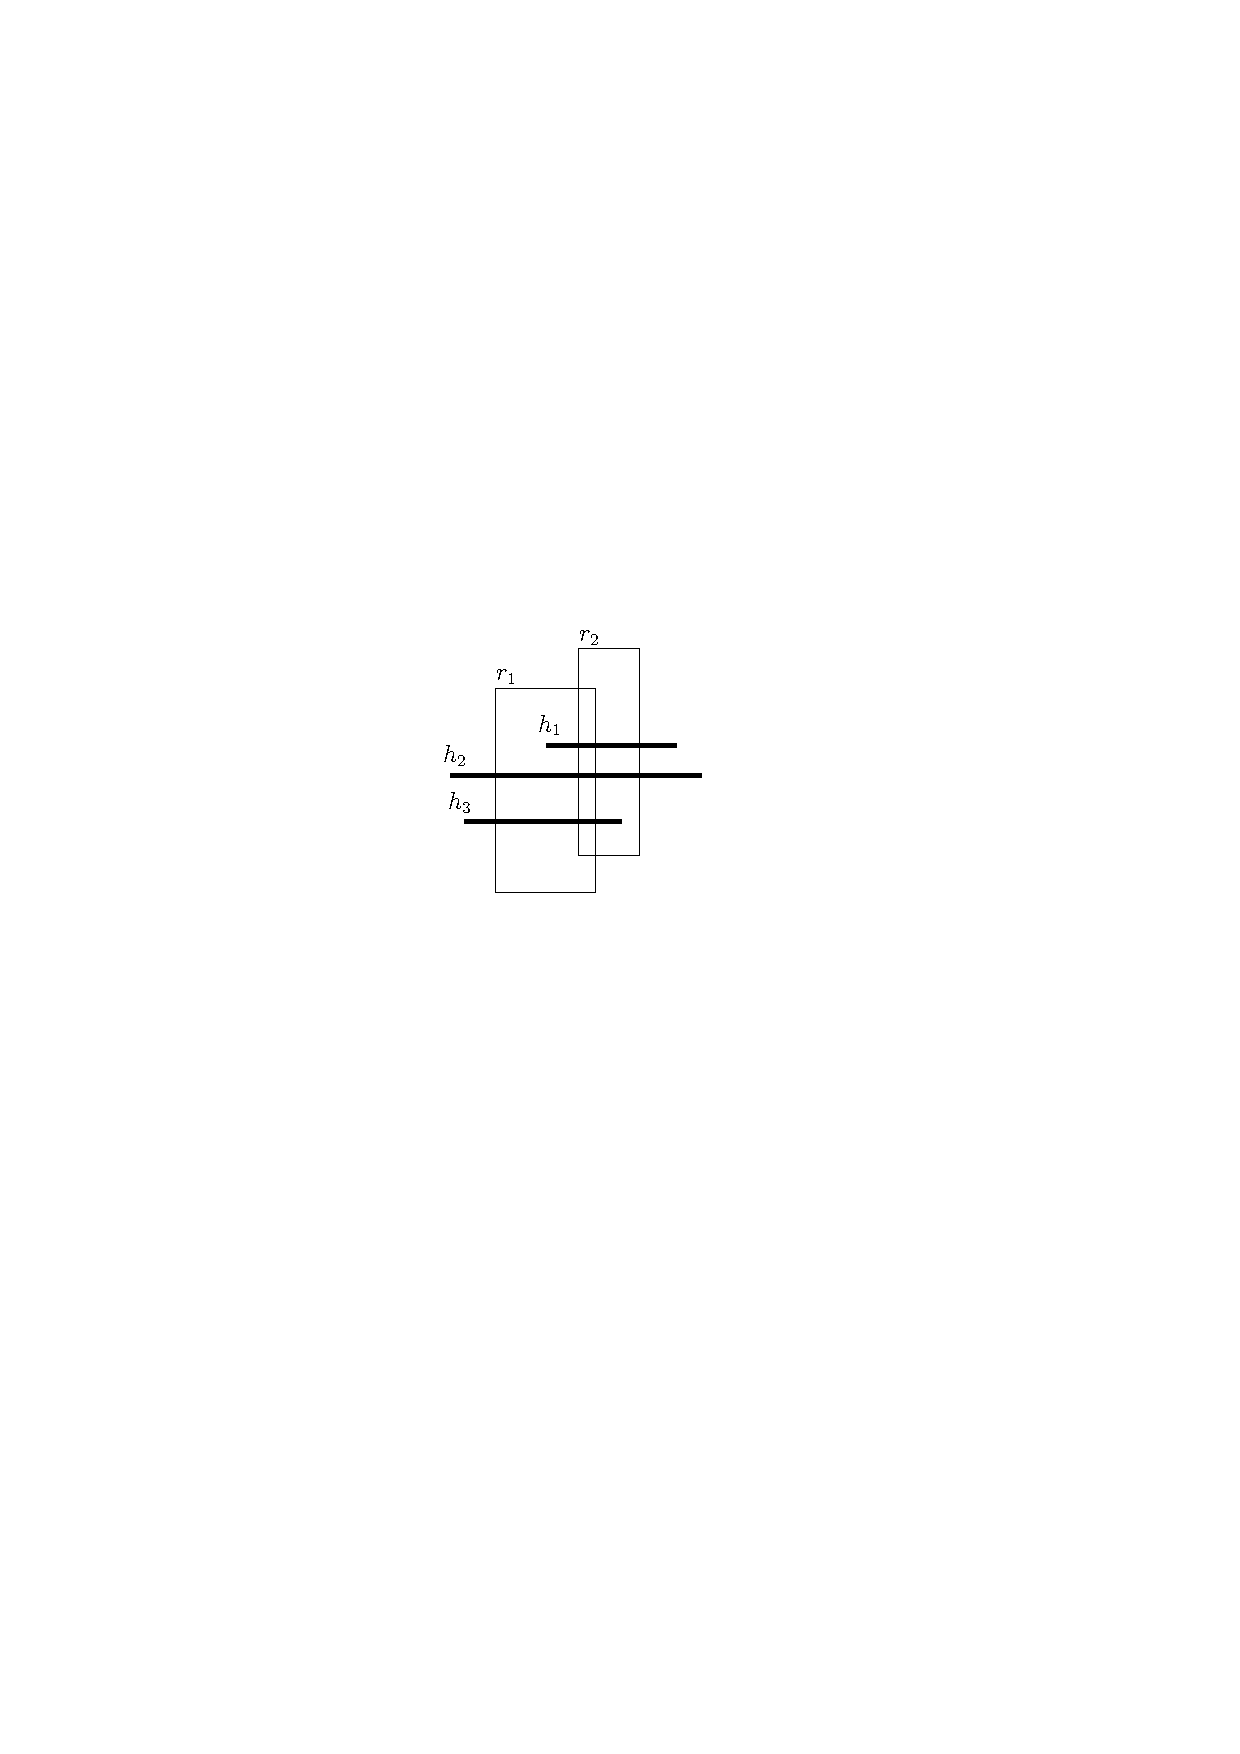
\includegraphics[height=30mm]{./artwork/prob-d} &
        \hspace{3mm}
        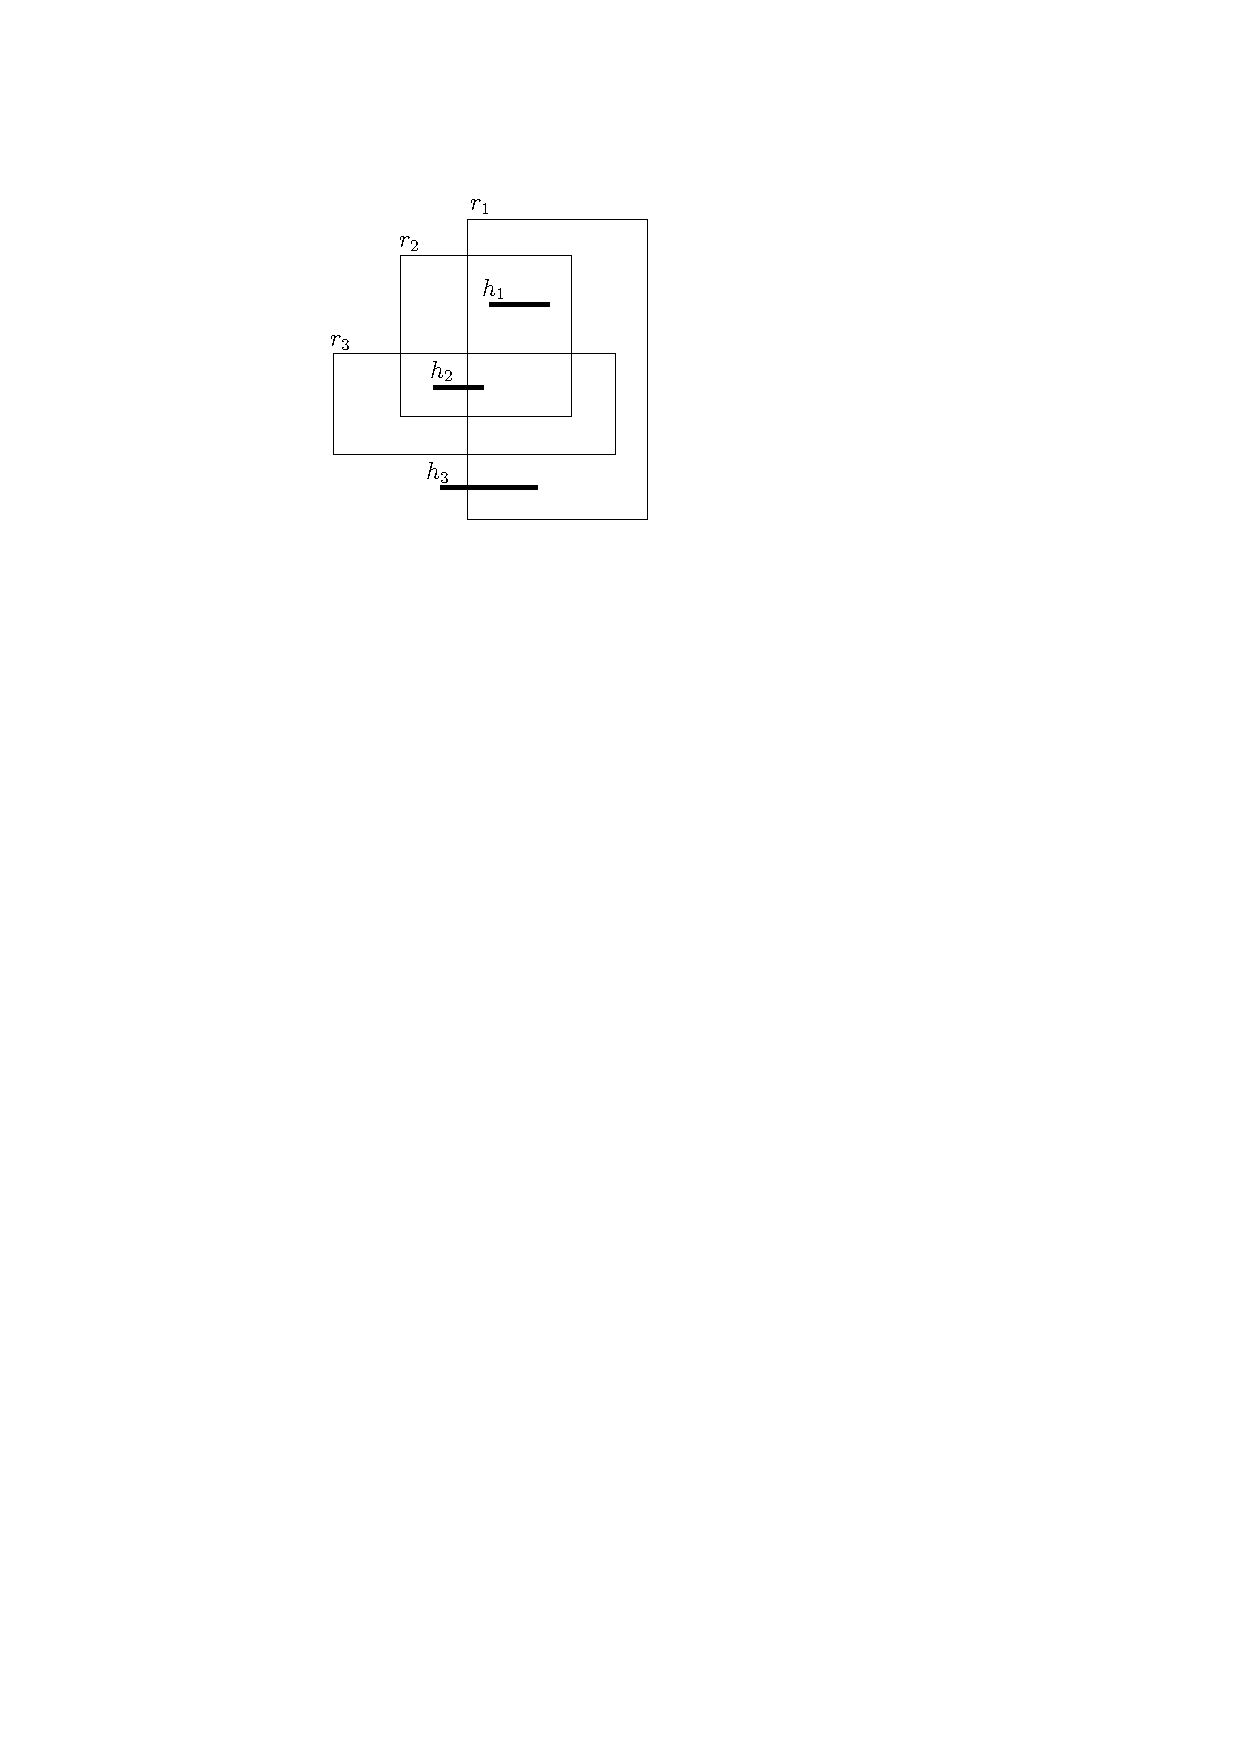
\includegraphics[height=30mm]{./artwork/prob-e} \\[2mm]
        (a) Problems $\mathscr{A}$ &
        \hspace{3mm}
        (b) Problem $\mathscr{B}$ &
        \hspace{3mm}
        (c) Problem $\mathscr{C}$ &
        \hspace{3mm}
        (d) Problem $\mathscr{D}$ &
        \hspace{3mm}
        (e) Problem $\mathscr{E}$
    \end{tabular}

    \figcapup
    \caption{Four geometric building brick problems}
    \label{fig:probs}
    \figcapdown
\end{figure*}

\section{Preliminaries in Geometry} \label{sec:bricks}

This section will first define some notions frequently used in our presentation and then introduce several  geometry problems, whose solutions will serve as building bricks for our $k$-SJ algorithm.

\extraspacing {\bf Terminology.} A {\em horizontal} segment is a segment of the form $[x_1, x_2] \times y$, and a {\em vertical} segment is a segment of the form $x \times [y_1, y_2]$. We say that a horizontal segment $h_1$ is {\em lower} (resp., {\em higher}) than another horizontal segment $h_2$ if the y-coordinate of $h_1$ is smaller (resp., larger) than that of $h_2$. Similarly, a vertical segment $v_1$ is {\em to the left} (resp., {\em right}) {\em of} another vertical segment $v_2$ if the x-coordinate of $v_1$ is smaller (resp., larger) than that of $v_2$.

\vgap

%Similarly, given a vertical segment $v$, we call a rectangle $r$ a {\em bottom-end covering rectangle} of $v$, if $r$ contains the bottom endpoint of $v$. \yf{need this?}

Given a horizontal segment $h = [x_1, x_2] \times y$, we call a rectangle $r$ a {\em left-end covering rectangle} of $h$, if $r$ contains the left endpoint of $h$ (i.e., $(x_1, y) \in r$). A horizontal/vertical segment $s$ {\em crosses} a rectangle $r$, if $s$ overlaps with $r$, but $r$ covers neither of the two endpoints of $s$. A rectangle $r$ {\em contains} a horizontal/vertical segment $s$, if $r$ covers both endpoints of $s$.

\vgap

Let $S$ be a set of segments where either all segments are horizontal or all are vertical. Given a rectangle $r$, we define 
\myeqn{
    \cross_S(r) = \{s \in S \mid \text{$s$ crosses $r$} \}. 
    \label{eqn:cross}
}
Let $R$ be a set of rectangles. Given a horizontal segment, we define 
\myeqn{
    \contained_R(h) = \{r \in R \mid \text{$h$ is contained in $r$} \}. 
    \label{eqn:contained}
}

Given a rectangle $r = [x_1, x_2] \times [y_1, y_2]$, we define $\xleft(r) = x_1$, $\xright(r) = x_2$, $\ybot(r) = y_1$, and $\ytop(r) = y_2$. Consider a $k$-tuple $\bm{t} = (r_1, r_2, ..., r_k)$ where $k \ge 2$, and each $\bm{t}[i] = r_i$ ($i \le [k]$) is a rectangle. We define 
\myeqn{
    B_\bm{t} &=& \cap_{i=1}^t r_i \label{eqn:B_t}
}
namely, $B_\bm{t}$ is the intersection of the rectangles in $\bm{t}$ (note: $B_\bm{t}$ is a rectangle itself). Let us introduce:
\myitems{
    \item $\gleft(\bm{t})$ as the rectangle $r_i$, $i \in [k]$, satisfying $\xleft(r_i)$ $= \xleft(B_\bm{t})$. In case multiple values in $[k]$ fulfill the condition, let $i$ be the smallest of such values.

    \item $\gbot(\bm{t})$ as the rectangle $r_i$, $i \in [k]$, satisfying $\ybot(r_i)$ $= \ybot(B_\bm{t})$. In case multiple values in $[k]$ fulfill the condition, let $i$ be the smallest of such values.
}
See Figure~\ref{fig:guard} for an illustration.

\extraspacing {\bf Problem $\bm{\mathscr{A}}$.} The input involves a set $P$ of 2D points and set $R$ of rectangles. In the {\em detection version} of Problem $\mathscr{A}$, the goal is to output, for each point $p \in P$, whether it is covered by at least one rectangle in $R$. Figure~\ref{fig:probs}a gives an example where $P = \set{p_1, p_2, p_3}$ and $R = \set{r_1, r_2}$; the output is ``yes'' for $p_2$ and $p_3$ and ``no'' for $p_1$. In Appendix~\ref{app:bricks}, we explain how to solve the problem in $O(n \log n)$ time, where $n = |P| + |R|$.

\vgap

In the {\em reporting version} of the problem, the goal is to output, for each point $p \in P$, all the rectangles $r \in R$ containing $p$, provided that at least one such $r$ exists. For example, in Figure~\ref{fig:guard}a, the output is $\set{(p_2: r_1, r_2), (p_3: r_2)}$. In Appendix~\ref{app:bricks}, we explain how to solve the problem in $O(n \log n + \out)$ time where $\out$ is the number of pairs $(p, r) \in P \times R$ such that $p \in r$.

\extraspacing {\bf Problem $\bm{\mathscr{B}}$.} The input involves a set $H$ of horizontal segments and a set $V$ of vertical segments, all in 2D space. The goal is to report, for each segment $h \in H$, the leftmost point $p$ on $h$ such that $p$ is on some vertical segment in $V$. If $h$ does not intersect with any segment in $V$, report nothing for $h$. Figure~\ref{fig:probs}b gives an example where $H = \set{h_1, h_2, h_3}$ and $V = \set{v_1, v_2}$; the output is $\set{(h_1, p_1), (h_2, p_2)}$. In Appendix~\ref{app:bricks}, we explain how to solve the problem in $O(n \log n)$ time where $n = |H| + |V|$.


\extraspacing {\bf Problem $\bm{\mathscr{C}}$.} The input involves a set $H$ of horizontal segments and a set $R$ of rectangles, all in 2D space. The goal is to report, for each segment $h \in H$, the rightmost point $p$ on $h$ satisfying the condition that $p$ is covered by at least one left-end covering rectangle of $h$ in $R$ --- formally, for $h = [x_1, x_2] \times y$, we aim to find the maximum $x \in [x_1, x_2]$ such that at least one rectangle $r \in R$ covers both the point $(x_1, y)$ and the point $(x, y)$. If the point $p$ exists (i.e., $h$ has at least one left-end covering rectangle in $R$), we should output a tuple $(h, p)$; otherwise, output nothing for $h$. Figure~\ref{fig:probs}c gives an example where $H = \set{h_1, h_2}$ and $R$ includes the three rectangles shown; the output is $\set{(h_1, p_1), (h_2, p_2)}$. In Appendix~\ref{app:bricks}, we explain how to solve the problem in $O(n \log n)$ time where $n = |H| + |R|$.

\extraspacing {\bf Problem $\bm{\mathscr{D}}$.} The input involves a set $H$ of horizontal segments and a set $R$ of rectangles, all in 2D space. In the {\em find-lowest} version of the problem, the goal is to report, for each rectangle $r \in R$, the lowest segment in $\cross_H(r)$ (see \eqref{eqn:cross}). If no segment in $H$ crosses $r$, output nothing for $r$.  Figure~\ref{fig:probs}d gives an example where $H = \set{h_1, h_2, h_3}$ and $R = \set{r_1, r_2}$; the output is $\set{(r_1, h_3), (r_2, h_2)}$. In Appendix~\ref{app:bricks}, we explain how to solve the problem in $O(n \log n)$ time where $n = |H| + |R|$.

\vgap

In the {\em find-all-sorted} version of the problem, the goal is to report, for each rectangle $r \in R$, the entire $\cross_H(r)$ sorted by y-coordinate. Formally, if $\cross_H(r) = \set{h_1, h_2, ..., h_z}$ (for some $z \ge 1$), we output $(r: h_1, h_2, ..., h_z)$, provided that $y_i \ge y_{i-1}$ for each $i \in [2, z]$ where $y_i$ (resp., $y_{i-1}$) is the y-projection of $h_i$ (resp., $h_{i-1}$). In the example of Figure~\ref{fig:probs}d, the output is $\set{(r_1: h_3, h_2), (r_2: h_2, h_1)}$. In Appendix~\ref{app:bricks}, we explain how to solve the problem in $O(n \log n + \out)$ time where $\out$ is the number of pairs $(h, r) \in H \times R$ such that $h$ crosses $r$.


\extraspacing {\bf Problem $\bm{\mathscr{E}}$.} The input involves a set $H$ of horizontal segments and a set $R$ of rectangles, all in 2D space. The goal is to report, for each segment $h \in H$, the set $\contained_R(h)$ --- defined in \eqref{eqn:contained} --- where the rectangles are sorted by their right boundaries. Formally, if $r_1, r_2, ..., r_z$ (for some $z \ge 1$) are all the rectangles in $\contained_R(h)$, we output $(h: r_1, r_2, ..., r_z)$, provided that $\xright(r_i) \ge \xright(r_{i-1})$ for each $i \in [2, z]$. Figure~\ref{fig:probs}e gives an example where $H = \set{h_1, h_2, h_3}$ and $R = \set{r_1, r_2, r_3}$; the output is $\set{(h_1: r_2, r_1), (h_2: r_2, r_3)}$. In Appendix~\ref{app:bricks}, we explain how to solve the problem in $O(n \log n + \out)$ time where $n = |H| + |R|$ and $\out$ is the number of pairs $(h, r) \in H \times R$ such that $r$ contains $h$.


\section{The Core: H-V Multiway Spatial Joins} \label{sec:hv}

Recall that the input of $k$-SJ comprises $k$ sets of rectangles: $R_1, R_2, ...,$ $R_k$. We now formulate a special version of $k$-SJ, named the {\em H-V $k$-SJ} problem. The special nature is reflected in the introduction of three constraints: (i) $k \ge 3$, (ii) $R_{k-1}$ should be a set of horizontal segments, and (iii) $R_k$ should be a set of vertical segments. For better clarity, we will represent the input sets as $R_1, R_2, ..., R_{k-2}, H$ ($=R_{k-1}$), and $V$ ($=R_k$). The goal is to output the join result $\J(R_1, ..., R_{k-2},$ $H, V)$, including every $k$-tuple $(r_1, ..., r_{k-2}, h, v) \in R_1 \times ... \times R_{k-2} \times H \times V$ such that $h \cap v \cap \bigcap_{i=1}^{k-2} r_i$ is not empty. 

%As we will see, conquering this sepcial version is the most challenging step in settling the original $k$-SJ problem optimally.

\vgap

Our objective is to prove that H-V $k$-SJ can be efficiently reduced to $(k-1)$-SJ --- note: it is $(k-1)$-SJ here, rather than H-V $(k-1)$-SJ. To facilitate our analysis, let us define the 1-SJ problem as follows: the input is a set $R$ of $n$ rectangles, and the goal is simply to enumerate each rectangle of $R$. The 1-SJ problem can be trivially ``solved'' in $O(n)$ time. We assume the existence of an algorithm $\A$ that can solve $\kappa$-SJ problems for all $\kappa \in [1, k-1]$. Denote by $F_\kappa(n, \out)$ the worst-case runtime of $\A$ on any instance of $\kappa$-SJ that has input size $n$ and output size $\out$. We consider that $F_\kappa(n, \out) \le F_{\kappa + 1}(n, \out)$ for any $\kappa \ge 1$, that is, its overhead on $\kappa$-SJ should not be larger than that on $(\kappa+1)$-SJ.

\vgap

We will establish:

\begin{lemma} \label{lmm:hv}
    Equipped with the algorithm $\A$ described above, the H-V $k$-SJ problem can be solved in time
    \myeqn{
        O(k) \cdot \big( F_{k-1}(n, \out) + n\log n + k \cdot \out \big) \nn
    }
    where $n$ (resp., $\out$) is the input (resp., output) size of the problem.
\end{lemma}

The part of the paper from this point till the end of Section~\ref{sec:hv:type2} will be devoted to proving the above lemma. This is the most challenging step in settling the general $k$-SJ problem optimally, as we will see in Section~\ref{sec:ksj}, where we will prove Theorems~\ref{thm:main-recur} and \ref{thm:main-alg} based on Lemma~\ref{lmm:hv}.

\vgap

%The condition is equivalent to saying that the intersection point of $h$ and $v$ falls in every $r_i$ of $i \in [k-2]$.


Consider any $k$-tuple $(r_1, ..., r_{k-2}, h, v)$ in the join result $\J(R_1, ...,$ $R_{k-2}, H, V)$. We classify the tuple into one of the two types below:

\myitems{
    \item {{\bf Type 1:}} $h$ crosses all of $r_1, ..., r_{k-2}$ and, at the same time, $v$ crosses all of $r_1, ..., r_{k-2}$; 
    
    \item {{\bf Type 2:}} either $h$ or $v$ fails to cross at least one rectangle in $\set{r_1, r_2, ..., r_{k-2}}$. Equivalently,
    there exists at least a rectangle $r_i$ (for some $i \in [k-2]$) that covers an endpoint of either $h$ or $v$ or both.
}
Figure~\ref{fig:hv:types} illustrates a result tuple of each type, assuming $k = 4$.

\vgap 

In Section~\ref{sec:hv:type1} (resp., \ref{sec:hv:type2}), we will explain how to produce the result tuples of Type 1 (resp., 2) in the time complexity claimed in Lemma~\ref{lmm:hv}.

\extraspacing {\bf Remark.} In \cite{rdr+11}, Rahul et al.\ studied the problem of storing a set $H$ of horizontal segments and a set $V$ of vertical segments in a data structure such that, given a query rectangle $r$, all the pairs $(h, v) \in H \times V$ satisfying $h \cap v \cap r \ne \emptyset$ can be reported efficiently. They developed a structure of $O(n \log n)$ space that can be built in $O(n \log n)$ time, and can be used to answer a query in $O(\log n + K)$ time, where $n = |H| + |V|$ and $K$ is the number of pairs reported. Their structure can be utilized to solve H-V 3-SJ in $O(n \log n + \out)$ time. We are unaware of a way to extend their solution to handle H-V $k$-SJ of $k > 3$. Our method for proving Lemma~\ref{lmm:hv} is based on fundamentally different ideas. 

\begin{figure}
    \begin{tabular}{cc}
        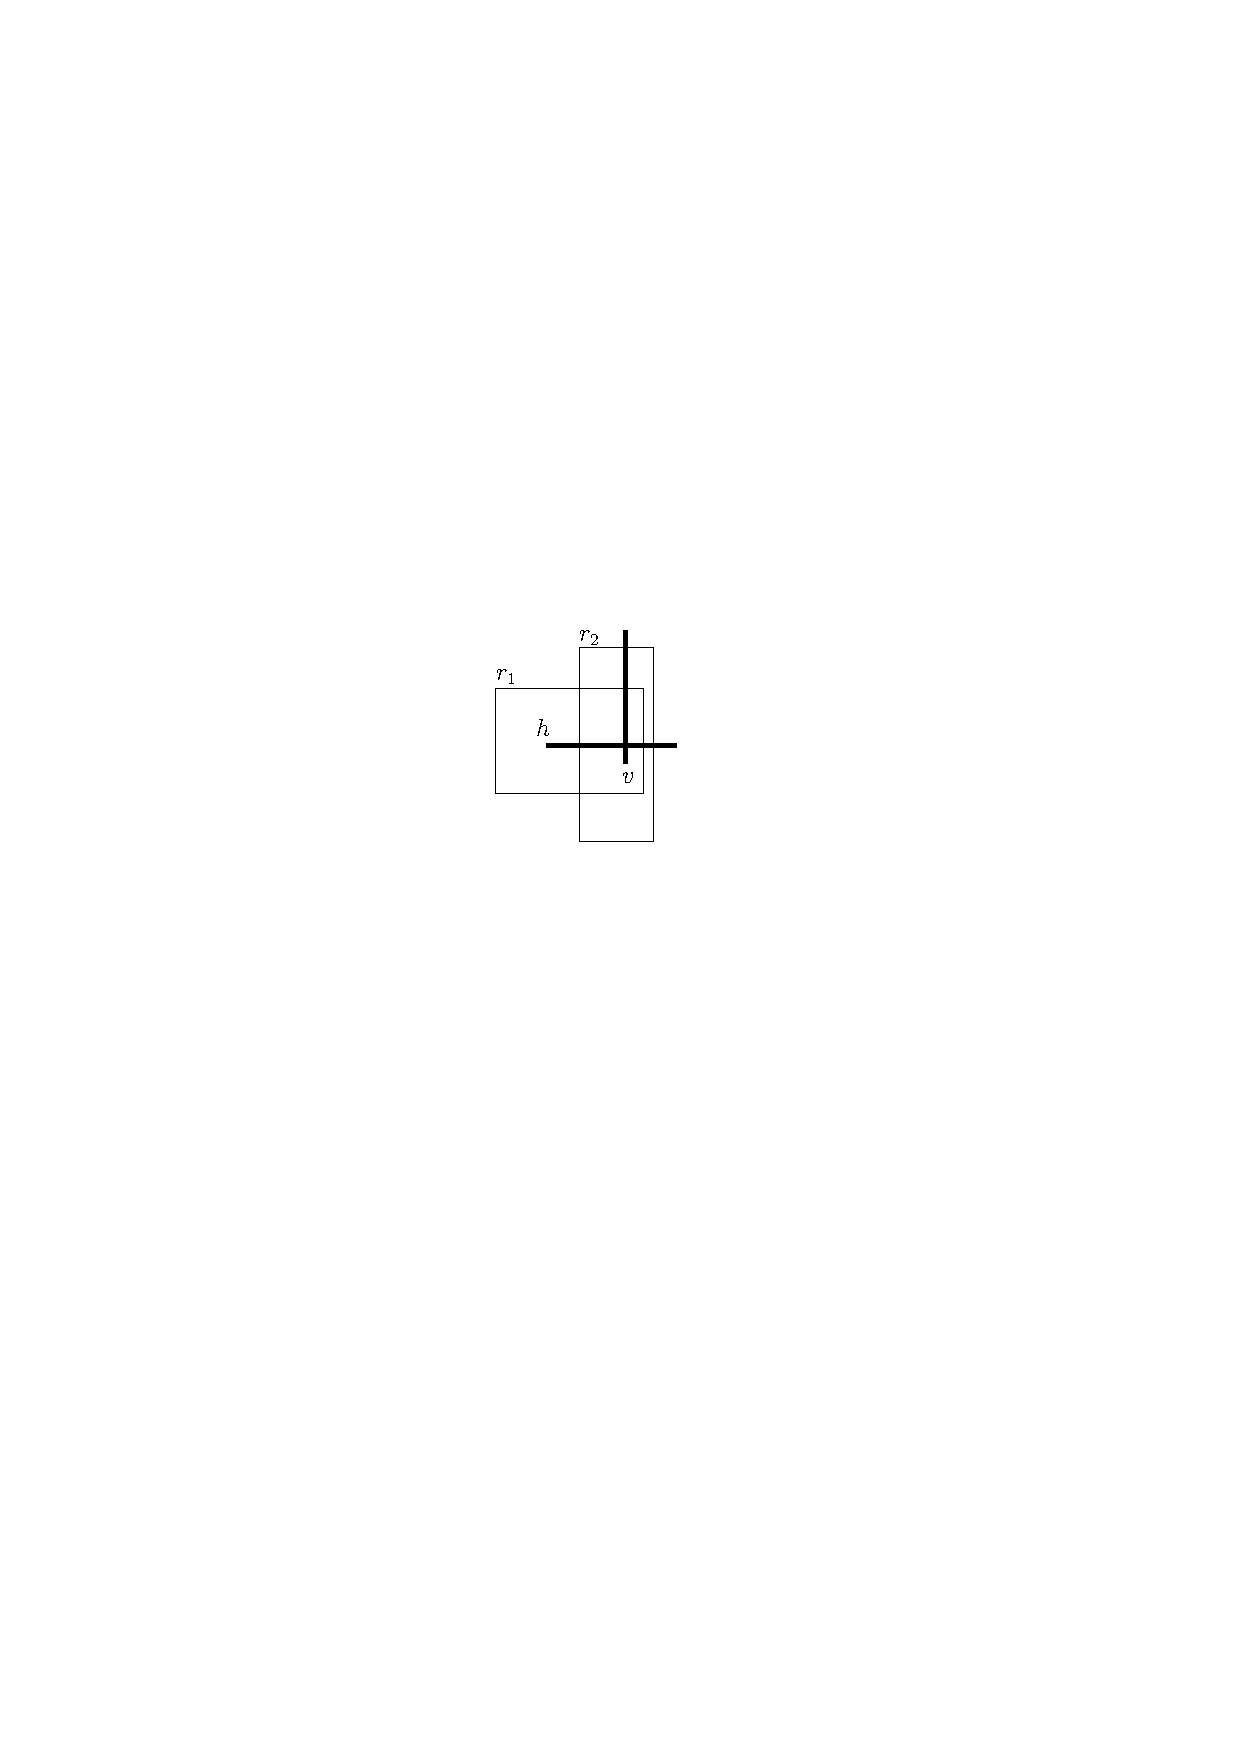
\includegraphics[height=23mm]{./artwork/type1} &
        \hspace{5mm} 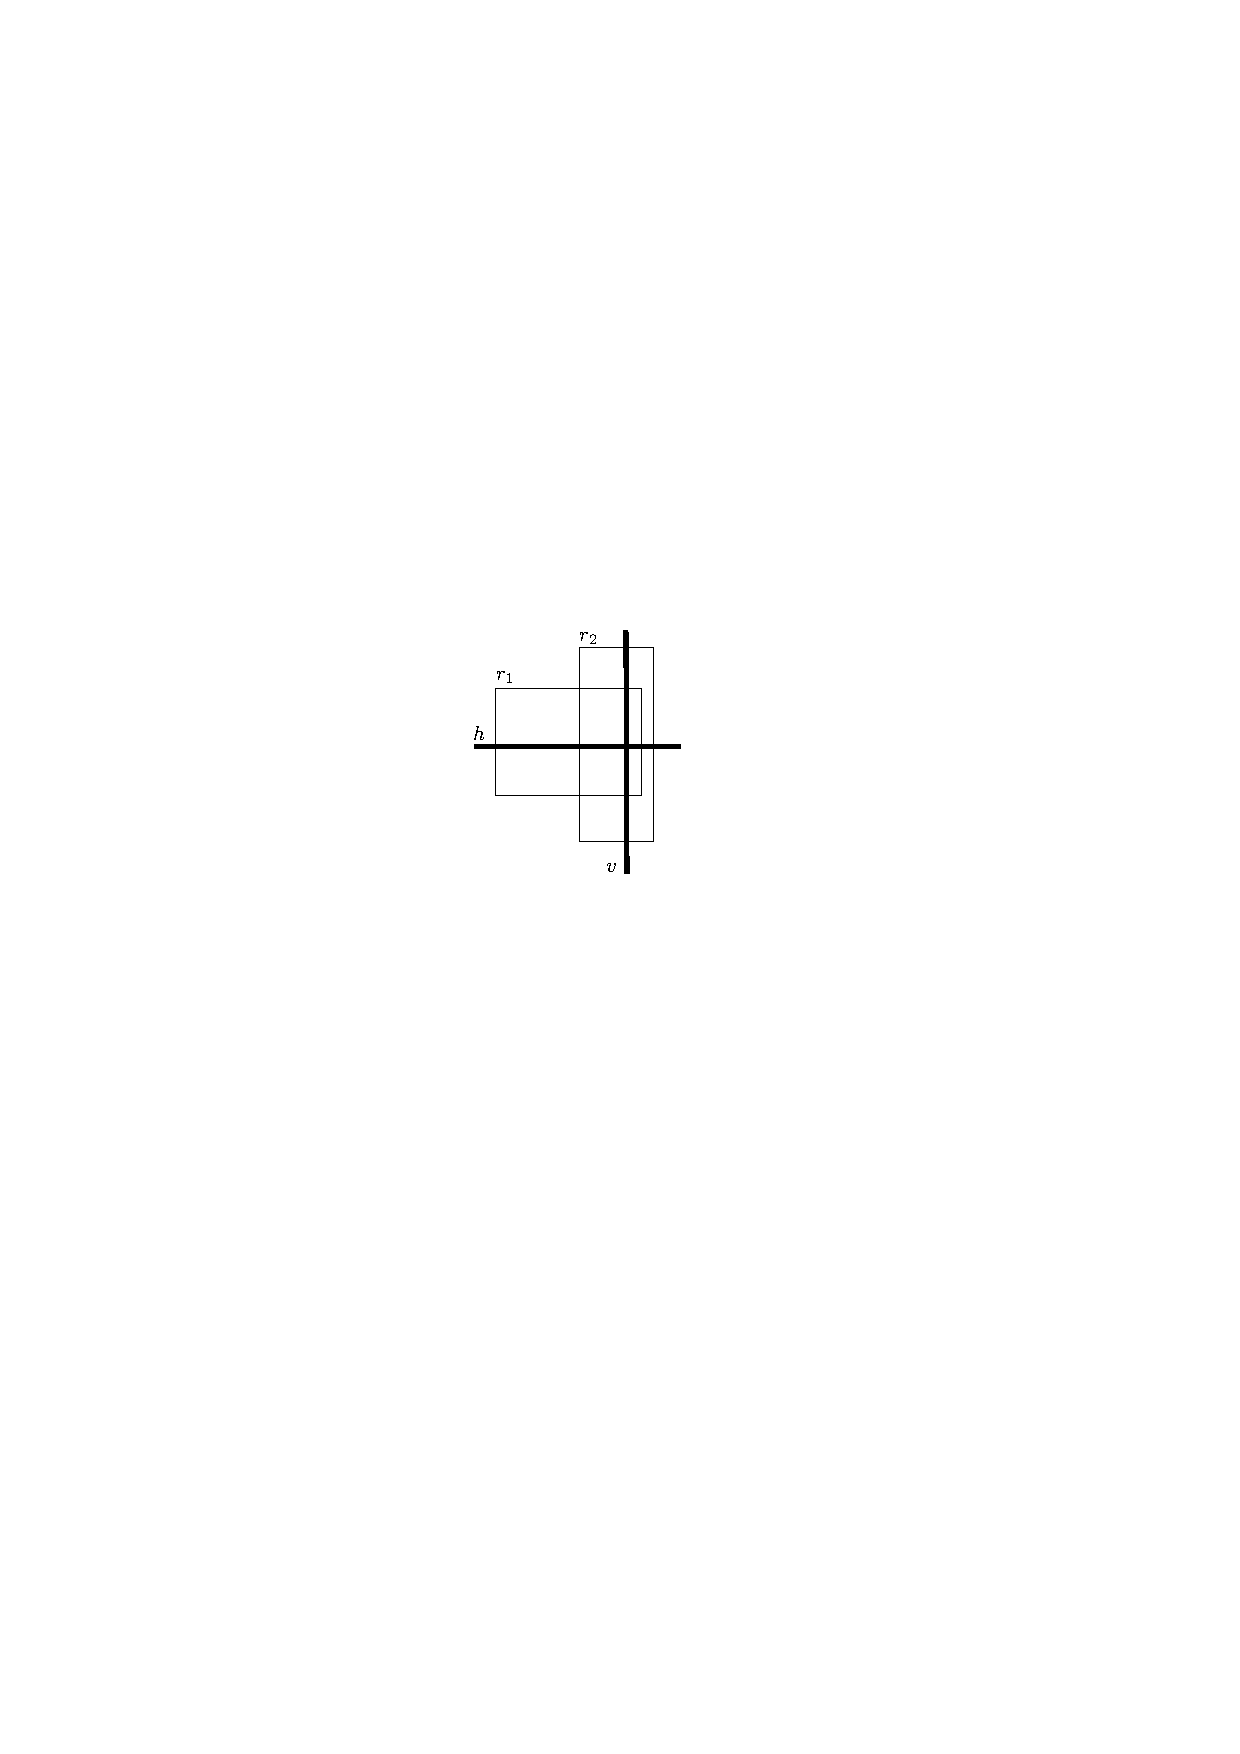
\includegraphics[height=27mm]{./artwork/type2} \\
        (a) Type 1 &
        (b) Type 2
    \end{tabular}

    \figcapup
    \caption{Classifying H-V $k$-SJ result tuples ($k$ = 4)}
    \label{fig:hv:types}
    \figcapdown
\end{figure}


\section{H-V $k$-SJ: Result Tuples of Type 1} \label{sec:hv:type1}

As before, let $R_1, ..., R_{k-2}, H$, and $V$ be the input sets of the H-V $k$-SJ problem. Denote by $\J_1$ the set of type-1 result tuples defined in Section~\ref{sec:hv}. In this section, we aim to compute a set $\J^*$ satisfying
\myeqn{
    \J_1
    \subseteq
    \J^*
    \subseteq
    \J(R_1, ..., R_{k-2}, H, V) \label{eqn:hv:type1:J*}
}
where $\J(R_1, ..., R_{k-2}, H, V)$, let us recall, is the join result of the (whole) H-V $k$-SJ. Remember that the output size $\out$ is defined to $|\J(R_1, ..., R_{k-2}, H, V)|$. From $\J^*$, we will report only those $k$-tuples belonging to $\J_1$ and ignore the rest. 

\extraspacing {\bf Sets $\bm{R_1', R_2', ..., R'_{k-2}}$.} Fix any $i \in [k-2]$. For each rectangle $r \in R_i$, we compute four segments:
\myitems{
    \item $h_1$ (resp., $h_2$): the lowest (resp., highest) segment in $H$ that crosses $r$;
    
    \item $v_1$ (resp., $v_2$): the leftmost (resp., rightmost) segment in $V$ that crosses $r$.
}
Define $r' = [x_1, x_2] \times [y_1, y_2]$, where $x_1$ (resp., $x_2$) is x-coordinate of $v_1$ (resp., $v_2$), and $y_1$ (resp., $y_2$) is y-coordinate of $h_1$ (resp., $h_2$). We say that $r'$ is the {\em trimmed rectangle} of $r$, and conversely, $r$ is the {\em full rectangle} of $r'$. Note that $r'$ exists if and only if $r$ is crossed by at least one horizontal segment in $H$ and by at least one vertical segment in $V$. 

%Moreover, it is possible for $h_1$ and $h_2$ to be the same segment; same for $v_1$ and $v_2$. 

\vgap 

Construct
\myeqn{
    R_i' &=& \set{r' \mid r \in R_i \text{ and its trimmed rectangle $r'$ exists}}. \nn
}
Computing the ``segment $h_1$'' for each $r \in R_i$ is an instance of Problem $\mathscr{D}$ (the find-lowest version, with $H$ and $R_i$ as the input). By symmetry, so is the computation of $h_2, v_1$, and $v_2$ segments for each $r \in R_i$. It thus follows from Section~\ref{sec:bricks} that $R_1', R_2', ..., R_{k-2}'$ can be produced in $O(n \log n)$ total time.

\vgap

We now solve a $(k-2)$-SJ problem with $R_1', R_2', ..., R_{k-2}'$ as the input using the algorithm $\A$ supplied (see Lemma~\ref{lmm:hv}). This $(k-2)$-SJ clearly has an input size at most $n$, and let us represent its result as $\J(R'_1, R'_2, ..., R'_{k-2})$. We prove in Appendix~\ref{app:hv}:

\begin{lemma} \label{lmm:hv:type1:recur-output}
    $|\J(R_1', R'_2, ..., R'_{k-2})| \le \out$.
\end{lemma}

We remind the reader that $\out$ is the output size of the original H-V $k$-SJ problem. As a corollary of Lemma~\ref{lmm:hv:type1:recur-output}, the $(k-2)$-SJ can be settled in $F_{k-2}(n, \out)$ time.

\yf{example}

\extraspacing {\bf Generating $\bm{\J^*}$.} Take any $(k-2)$-tuple $\bm{t} = (r'_1, r'_2, ...,$ $r'_{k-2}) \in \J(R_1', R'_2, ..., R'_{k-2})$. The reader should recall from Section~\ref{sec:bricks} that
\myitems{
    \item $B_\bm{t}$ is $\bigcap_{i=1}^{k-2} \bm{t}[i] = \bigcap_{i=1}^{k-2} r'_i$;
    \item $\gleft(\bm{t})$ is the $r'_i$ ($1 \le i \le k-2$) with $\xleft(r'_i) = \xleft(B_\bm{t})$;
    \item $\gbot(\bm{t})$ is the $r'_i$ ($1 \le i \le k-2$) with $\ybot(r'_i) = \ybot(B_\bm{t})$.
}
We now introduce:
\myeqn{
    \dcross_H(\bm{t}) = \set{h \in H \mid \text{$h$ crosses both $B_\bm{t}$ and $\gbot(\bm{t})$}} \label{eqn:dcross-H} \\
    \dcross_V(\bm{t}) = \set{v \in V \mid \text{$v$ crosses both $B_\bm{t}$ and $\gleft(\bm{t})$}}. \nn
    %\label{eqn:dcross-H} 
}
The prefix ``d-'' stands for ``double''. These sets have important properties as stated in the next lemma, whose proof can be found in Appendix~\ref{app:hv}:

\begin{lemma} \label{lmm:hv:type1:properties}
    %Let $r_i$ be the full rectangle of $r_i'$ for each $i \in [k-2]$.
    All the following statements are true:
    \myenums{
        \item Consider any $(k-2)$-tuple $\bm{t} \in \J(R_1', R'_2, ..., R'_{k-2})$. Let $r_i$ ($i$ $\in$  $[k-2]$) be the full rectangle of $\bm{t}[i]$. Then, for any $h \in \dcross_H(\bm{t})$ and any $v \in \dcross_V(\bm{t})$, the $k$-tuple $(r_1, r_2,$ $...,$ $r_{k-2}, h, v)$ must belong to $\J(R_1, ..., R_{k-2}, H, V)$.
        
        \item Consider any a $k$-tuple $(r_1, r_2, ..., r_{k-2}, h, v) \in \J_1$. Let $r'_i$ ($i \in [k-2])$ be the trimmed rectangle of $r_i$, and set $\bm{t} = (r'_1, r'_2, ...,$ $r'_{k-2})$. Then, we must have 
        \myitems{
            \item $\bm{t} \in \J(R_1', R'_2, ..., R'_{k-2})$;
            \item $h \in \dcross_H(\bm{t})$ and $v \in \dcross_V(\bm{t})$. 
        }
        
        \vspace{2mm}
        
        \item $\sum_{\bm{t}} |\dcross_H(\bm{t})| \le \out$ and $\sum_{\bm{t}} |\dcross_V(\bm{t})| \le \out$, where the two summations are over all $\bm{t} \in \J(R_1', R'_2, ..., R'_{k-2})$.
    }
\end{lemma}

\yf{example}

\vgap 

Equipped with Lemma~\ref{lmm:hv:type1:properties}, we generate our target $\J^*$ as follows:

\mytab{
    \> {\bf algorithm generate-$\J^*$} \\
    \> 1.\> $\J^* = \emptyset$ \\
    \> 2.\> {\bf for} each $(k-2)$-tuple $\bm{t} \in \J(R'_1, ..., R'_{k-2})$ {\bf do} \\
    \> 3.\>\> $r_i \leftarrow$ the full rectangle of $\bm{t}[i]$, for each $i \in [k-2]$ \\
    \> 4.\>\> {\bf for} each $(h, v) \in \dcross_H(\bm{t}) \times \dcross_V(\bm{t})$ {\bf do} \\
    \> 5.\>\>\> add $(r_1, ..., r_{k-2}, h, v)$ to $\J^*$
}


By statements (1) and (2) of Lemma~\ref{lmm:hv:type1:properties}, the set $\J^*$ thus computed indeed satisfies \eqref{eqn:hv:type1:J*}. Furthermore, if we are given $\dcross_H(\bm{t})$ and $\dcross_V(\bm{t})$ for each $\bm{t}$, the above algorithm runs in $O(1 + |\J(R'_1, ..., R'_{k-2})| + k \cdot |\J^*|) = O(1 + k \cdot \out)$ time, where the derivation used \eqref{eqn:hv:type1:J*} and Lemma~\ref{lmm:hv:type1:recur-output}.

\vgap 

The rest of the section will focus on how to prepare the sets $\dcross_H(\bm{t})$ of all $\bm{t} \in \J(R_1', ..., R_{k-2}')$ in $O(n \log n + k \cdot \out)$ time. An analogous method can be used to compute the sets $\dcross_V(\bm{t})$ of all $\bm{t}$ in the same time complexity.

\extraspacing {\bf Sets $\bm{R^*_1, R^*_2, ..., R^*_{k-2}}$.} Fix any $i \in [k-2]$. For each rectangle $r' \in R_i'$, define
\myeqn{
    \maxtop(r') &=& \max_{\bm{t} \in \J(R'_1, ..., R'_{k-2}): \gbot(\bm{t}) = r'} \ytop(B_\bm{t}). 
}
We set $\maxtop(r')$ to $-\infty$, if no $\bm{t} \in \J(R'_1, ..., R'_{k-2})$ has $r'$ as the $\gbot(\bm{t})$. When $\maxtop(r') \ne -\infty$, assuming $r' = [x_1, x_2] \times [y_1, y_2]$, we introduce a rectangle
\myeqn{
    r^* &=& [x_1, x_2] \times [y_1, \maxtop(r')]. \nn
}
and call it the {\em top-sliced rectangle} of $r'$.

\vgap

\yf{example}

\vgap 

Next, we construct from $R_i'$ a new set of rectangles: 
\myeqn{
    R^*_i = \set{r^* \mid r' \in R_i' \text{ and its top-sliced rectangle $r^*$ exists}}. \label{eqn:hv:type1:R*}
}
In Appendix~\ref{app:hv}, we show how to compute produce $R^*_1, ..., R^*_{k-2}$ together in $O(n + k \cdot \out)$ total time.

\vgap 

Our focus lies specifically on the sets $\cross_H(r^*)$ of the rectangles $r^*$ in $R^*_i$, where $\cross_H(r^*)$ --- defined in \eqref{eqn:cross} --- is the set of segments in $H$ crossing $r^*$. The following lemma, proven in Appendix~\ref{app:hv}, presents some useful properties of these sets. 

\begin{lemma} \label{lmm:hv:type1:cross-r*}
    Both statements below are true: 
    \myenums{
        \item $\sum_{i=1}^k \sum_{r^* \in R^*_i} |\cross_H(r^*)| \le \out$.
        
        \item Consider any tuple $\bm{t} \in \J(R'_1, ..., R'_{k-2})$. Let $r' = \gbot(\bm{t})$ and $r^*$ be the top-sliced rectangle of $r'$. Then, we have $\dcross_H(\bm{t})$ $\subseteq \cross_H(r^*)$. Furthermore, if the (horizontal) segments of $\cross_H(r^*)$ are sorted in ascending order of y-coordinate, then $\dcross_H(\bm{t})$ includes a prefix of the sorted order.
    }
\end{lemma}

\yf{example}

Finding the $\cross_H(r^*)$ sets of all $r^* \in R^*_i$ is an instance of the find-all-sorted version of Problem $\mathscr{D}$ (with $H$ and $R^*_i$ as the input). Statement (1) of Lemma~\ref{lmm:hv:type1:cross-r*}, as well as the discussion in Section~\ref{sec:bricks}, assures us that the total time to do so for all $R^*_1, ..., R^*_{k-2}$ is bounded by $O(n \log n + \out)$. Note that, for each $\cross_H(r^*)$ computed, the (horizontal) segments therein has been sorted in ascending order of y-coordinate.


\extraspacing {\bf Computing the ``d-cross'' Sets.} We are ready to compute $\dcross_H(\bm{t})$, defined in \eqref{eqn:dcross-H}, for any $\bm{t} \in \J(R'_1, ..., R'_{k-2})$, thanks to Statement (2) of Lemma~\ref{lmm:hv:type1:cross-r*}. First, compute $B_\bm{t}$, obtain the rectangle $r' = \gbot(\bm{t})$, and fetch the (already computed) top-sliced rectangle $r^*$ of $r'$; these steps require $O(k)$ time. Then, scan the segments in $\cross_H(r^*)$ in ascending order of their y-coordinates. For each segment $h$ scanned, check whether $h$ belongs to $\dcross_H(\bm{t})$, namely, whether $h$ crosses $B_\bm{t}$ (the reader can verify that $h$ must cross $\gbot(\bm{t})$); this can be done in constant time. Abort the scan as soon as $h \notin \dcross_H(\bm{t})$. This way, we produce $\dcross_H(\bm{t})$ in $O(k + |\dcross_H(\bm{t})|)$ time. Doing so for all $\bm{t} \in \J(R'_1, ..., R'_{k-2})$ takes $O(k \cdot |\J| + \sum_\bm{t} |\dcross_H(t)|) = O(k \cdot \out)$ time, where the derivation used Lemma~\ref{lmm:hv:type1:recur-output} and statement (3) of Lemma~\ref{lmm:hv:type1:properties}.

\vgap 

We conclude that $\J_1$ --- the set of type-1 result tuples --- can be computed in $F_{k-2}(n, \out) + O(n \log n +  k \cdot \out)$ time.

\section{H-V $k$-SJ: Result Tuples of Type 2} \label{sec:hv:type2}

Still, denote by $R_1, ..., R_{k-2}, H$, and $V$ the input sets of the H-V $k$-SJ problem. This section will explain how to find the result tuples of Type 2 as defined in Section~\ref{sec:hv}.

\vgap

As mentioned before, for a result tuple $(r_1, ..., r_{k-2}, h, v)$ of this type, a rectangle $r_i$, for some $i \in [k-2]$, covers an endpoint of $h$ or $v$ or both. As (i) there are $k-2$ choices for $i$ and (ii) $h$ and $v$ together have four endpoints, we can divide Type 2 further into $4(k-2)$ ``sub-types'': in subtype 1 (resp., 2), $r_1$ covers the left (resp., right) endpoint of $h$, in subtype 3 (resp., 4), $r_1$ covers the bottom (resp., top) endpoint of $v$, in subtype 5 (resp., 6), $r_2$ covers the left (resp., right) endpoint of $h$, etc. It is possible for the result tuple to belong to multiple sub-types simultaneously.

\vgap 

Next, we will focus on producing the result tuples of a particular sub-type: those tuples $(r_1, ..., r_{k-2}, h, v)$ where $r_{k-2}$ covers the left endpoint of $h$ --- let us denote this set of result tuples as $\J_2$. Other sub-types can be computed using the same algorithm, by symmetry.

\vgap

A remark is in order about duplicate removal. By finding each sub-type separately, we may see the same result tuple multiple times (precisely, up to $4(k-2)$ times) in the whole algorithm. However, this does not mean that the tuple needs to be reported multiple times. Whenever a type-2 result tuple is found, we can immediately decide in $O(k)$ time all the sub-types it belongs to. To avoid outputting the tuple more than once, we can enforce a policy to designate a specific sub-type for outputting. One such policy is the following: among all sub-types that the tuple belongs to, identify the one with the smallest sub-type number $t$ (an integer from 1 to $4(k-2)$); report the tuple only when we are computing the particular sub-type $t$.

\extraspacing {\bf Set $\bm{H'}$.} Take any horizontal segment $h = [x_1, x_2] \times y \in H$. Let $p$ be the rightmost point $p$ on $h$ satisfying the condition that at least one rectangle in $R_{k-2}$ covers $p$. This point $p$ exists if and only if $h$ has at least one left-end covering rectangle in $R_{k-2}$. If $p$ exists and has coordinates $(x, y)$, we refer to the segment $h' = [x_1, x] \times y$ as the {\em trimmed segment} of $h$; conversely, we call $h$ the {\em full segment} of $h'$. 

\vgap 

Construct
\myeqn{
    H' &=& \{h' \mid h \in H \text{ and its trimmed segment $h'$ exists} \}. \nn
}
The construction is an instance of Problem $\mathscr{C}$ (with $H$ and $R_{k-2}$ as the input) and finishes in $O(n \log n)$ time based on the discussion in Section~\ref{sec:bricks}.

\vgap 

Now, solve a $(k-1)$-SJ problem with $R_1, ..., R_{k-3}, H', V$ as the input using the algorithm $\A$ supplied (see Lemma~\ref{lmm:hv}). Let $\J(R_1, ...,$ $R_{k-3}, H', V)$ represent the result of this $(k-1)$-SJ, whose input size is at most $n$. Given the lemma below (which is proved in Appendix~\ref{app:hv}), we assert that $\J(R_1, ..., R_{k-3}, H', V)$ can be computed in $F_{k-1}(n, \out)$ time.

\begin{lemma} \label{lmm:hv:type2:recur-output}
    $|\J(R_1, ..., R_{k-3}, H', V)| \le \out$.
\end{lemma}



\yf{example}

\extraspacing {\bf Generating $\bm{\J_2}$.} Take any $(k-1)$-tuple $\bm{t} = (r_1, ..., r_{k-3}, h', v) \in \J(R_1, ..., R_{k-3}, H', V)$. Observe that $B_\bm{t}$ --- defined in \eqref{eqn:B_t} --- is a point (due to $h'$ and $v$). Suppose $h' = [x_1, x_2] \times y$ and $B_\bm{t} = (x, y)$, we define the {\em effective horizontal segment} of $\bm{t}$ as the horizontal segment $[x_1, x] \times y$. 

\vgap

Define
\myeqn{
    \contained_{R_{k-2}}(\bm{t}) &=& \{r \in R_{k-2} \mid \text{ the effective horizontal } \nn \\[-1mm]
    && \text{segment of $\bm{t}$ is contained in $r$}   \}
    \label{eqn:type2:contained-t}
}
The above should not be confused with \eqref{eqn:contained}, where the ``$\contained$'' function takes a segment as the input, rather than a tuple.

\vgap 

We prove the next lemma in Appendix~\ref{app:hv} (to avoid confusion, the reader may want to be reminded that, for each $\bm{t} \in \J(R_1, ..., R_{k-3}, H', V)$, $\bm{t}[k-2]$ is a horizontal segment and $\bm{t}[k-1]$ is a vertical segment).

\begin{lemma} \label{lmm:hv:type2:properties}
    All the following statements are true:
    \myenums{
        \item Consider any $(k-1)$-tuple $\bm{t} \in \J(R_1, ..., R_{k-3}, H', V)$. Denote by $h$ the full segment of $\bm{t}[k-2]$. Then, for any $r \in \contained_{R_{k-2}}(\bm{t})$, the $k$-tuple $(\bm{t}[1], ..., \bm{t}[k-3], r, h, \bm{t}[k-1])$ must belong to $\J_2$.
        
        \item Consider any $k$-tuple $(r_1, ..., r_{k-2}, h, v) \in \J_2$. Let $h'$ be the trimmed segment of $h$, and set $\bm{t} = (r_1, ..., r_{k-3}, h', v)$. Then, $\bm{t} \in \J(R_1, ..., R_{k-3}, H', V)$ and $h' \in \contained_{R_{k-2}}(\bm{t})$.
        
        \item $\sum_{\bm{t}} |\contained_{R_{k-2}}(\bm{t})| \le \out$, where the summation is over all $\bm{t} \in \J(R_1, ..., R_{k-3}, H', V)$.
    }
\end{lemma}


Equipped with Lemma~\ref{lmm:hv:type1:properties}, we generate our target $\J_2$ as follows:

\mytab{
    \> {\bf algorithm generate-$\J_2$} \\
    \> 1.\> $\J_2 = \emptyset$ \\
    \> 2.\> {\bf for} each $(k-2)$-tuple $\bm{t} \in \J(R_1, ..., R_{k-3}, H', V)$ {\bf do} \\
    \> 3.\>\> $h \leftarrow$ the full segment of $\bm{t}[k-2]$ \\
    \> 4.\>\> {\bf for} each $r \in \contained_{R_{k-2}}(\bm{t})$ {\bf do} \\
    \> 5.\>\>\> add $(\bm{t}[1], ..., \bm{t}[k-3], r, h, \bm{t}[k-1])$ to $\J_2$
}

The correctness of the algorithm follows from statements (1) and (2) of Lemma~\ref{lmm:hv:type2:properties}. Furthermore, if we are given $\contained_{R_{k-2}}(\bm{t})$ for each $\bm{t}$, statement (3) of assures us that the algorithm runs in $O(1 + |\J(R_1, ..., R_{k-3}, H', V)| + k \sum_\bm{t} |\contained_{R_{k-2}}(\bm{t})|) = O(1 + k \cdot \out)$ time, where the derivation used Lemma~\ref{lmm:hv:type2:recur-output} and statement (3) of Lemma~\ref{lmm:hv:type2:properties}.


\extraspacing {\bf Set $\bm{H^*}$.} 
For each segment $h' \in H'$, define
\myeqn{
    \minleft(h') = \min_{\substack{\text{$\bm{t} \in \J(R_1, ..., R_{k-3}, H', V):$}\\ \text{$\bm{t}[k-2] = h'$}}} \text{$x$-coordinate of $\bm{t}[k-1]$}. 
    \label{eqn:minleft}
}
We set $\minleft(h')$ to $\infty$, if no $\bm{t} \in \J(R_1, ..., R_{k-3}, H', V)$ has $h'$ in its field $\bm{t}[k-2]$. When $\minleft(h') \ne \infty$, assuming $h' = [x_1, x_2] \times y$, we introduce a horizontal segment
\myeqn{
    h^* &=& [x_1, \minleft(h')] \times y. \nn
}
and call it the {\em minimal segment} of $h'$.

\vgap

\yf{example}

\vgap 

Next, we construct a new set of horizontal segments: 
\myeqn{
    H^* = \set{h^* \mid h' \in H' \text{ and its minimal segment $h^*$ exists}}. \label{eqn:hv:type2:H*}
}
This can be done in $O(n + k \cdot \out)$ time, as shown in Appendix~\ref{app:hv}. 

%Computing $H^*$ from $H'$ and $V$ is an instance of Problem $\mathscr{B}$, and can be achieved in $O(n \log n)$ as per the discussion from Section~\ref{sec:bricks}. 

\vgap 

We will utilize the sets $\contained_{R_{k-2}}(h^*)$ of the segments $h^*$ in $H^*$, where $\contained_{R_{k-2}}(h^*)$ --- defined in \eqref{eqn:contained} --- is the set of rectangles in $R_{k-2}$ containing $h^*$. These sets have some useful properties:

\begin{lemma} \label{lmm:hv:type2:contained-h*}
    Both statements below are true: 
    \myenums{
        \item $\sum_{h^* \in H^*} |\contained_{R_{k-2}}(h^*)| \le \out$.
        
        \item Consider any tuple $\bm{t} \in \J(R_1, ..., R_{k-3}, H', V)$. Set $h' = \bm{t}[k-2]$ and let $h^*$ be the minimal segment of $h'$. Then, $$\contained_{R_{k-2}}(\bm{t}) \subseteq \contained_{R_{k-2}}(h^*).$$ Furthermore, if the rectangles $r$ in $\contained_{R_{k-2}}(h^*)$ are sorted in descending order of $\xright(r)$, then $\contained_{R_{k-2}}(\bm{t})$ includes a prefix of the sorted order.
    }
\end{lemma}

The proof can be found in Appendix~\ref{app:hv}. 

\yf{example}

Finding the $\contained_{R_{k-2}}(h^*)$ sets of all $h^* \in H^*$ is an instance of the find-all-sorted version of Problem $\mathscr{E}$ (with $H^*$ and $R_{k-2}$ as the input). The cost is $O(n \log n + \out)$ according statement (1) of Lemma~\ref{lmm:hv:type1:cross-r*} and the discussion in Section~\ref{sec:bricks}. Note that, for each $\contained_{R_{k-2}}(h^*)$ computed, the rectangles $r$ therein have been sorted in descending order of $\xright(r)$.


\extraspacing {\bf Computing the ``$\bm{\contained_{R_{k-2}}(t)}$'' Sets.} Statement (2) of Lemma~\ref{lmm:hv:type2:contained-h*} allows us to produce $\contained_{R_{k-2}}(h^*)$, defined in \eqref{eqn:type2:contained-t}, for each $\bm{t} \in \J(R_1, ..., R_{k-3}, H', V)$ as follows. First, fetch the (already computed) minimal segment $h^*$ of $\bm{t}[k-2]$ in $O(1)$ time. Then, scan the rectangles $r$ of $\contained_{R_{k-2}}(h^*)$ in descending order of $\xright(r)$. For each $r$ scanned, check whether $r \in \contained_{R_{k-2}}(\bm{t})$, or equivalently, whether $r$ covers $B_\bm{t}$ (recall that $B_\bm{t}$ is a point); the cost for such a check is $O(1)$. Abort the scan as soon as $r \notin 
\contained_{R_{k-2}}(\bm{t})$. This way, $\contained_{R_{k-2}}(t)$ can be decided in $O(k + |\contained_{R_{k-2}}(\bm{t})|)$ time. Doing so for all $\bm{t} \in \J(R_1, ..., R_{k-3},$ $H', V)$ takes $O(k \cdot |\J| + \sum_\bm{t} |\contained_{R_{k-2}}(\bm{t})|) = O(k \cdot \out)$ time, where the derivation used Lemma~\ref{lmm:hv:type2:recur-output} and statement (3) of Lemma~\ref{lmm:hv:type2:properties}.



\vgap 

We conclude that $\J_2$ --- the set of type-2 result tuples $(r_1, ..., r_{k-2},$ $h, v)$ where $r_{k-2}$ covers the left endpoint of $h$ --- can be computed in $F_{k-1}(n, \out) + O(n \log n +  k \cdot \out)$ time. Remember that, to generate the entire type-2 result, we need to repeat the algorithm $4(k-2)$ times (one for each sub-type). The total running time is therefore $O(k) \cdot (F_{k-1}(n, \out) + n \log n +  k \cdot \out)$, as claimed in Lemma~\ref{lmm:hv}.

\begin{figure}
    \begin{tabular}{cc}
        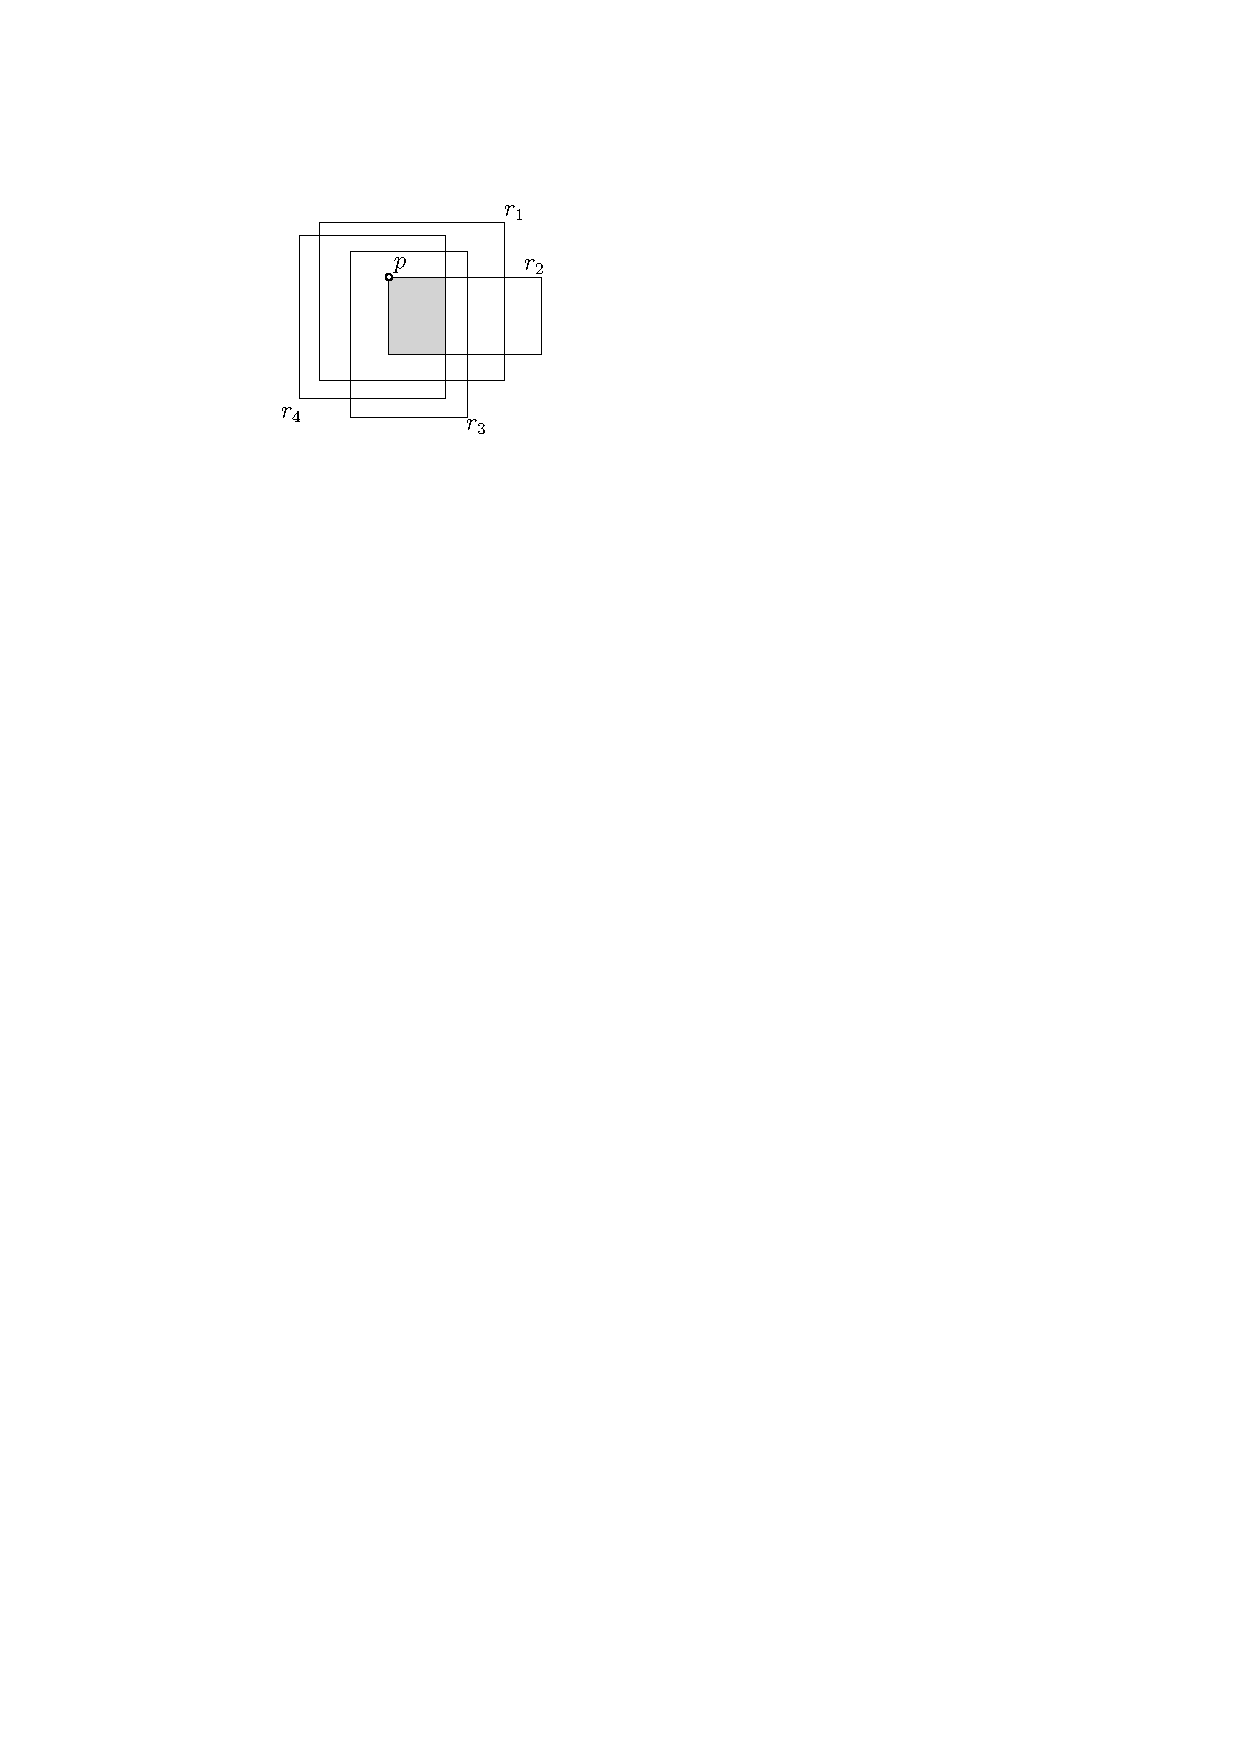
\includegraphics[height=27mm]{./artwork/cat1} &
        \hspace{5mm} 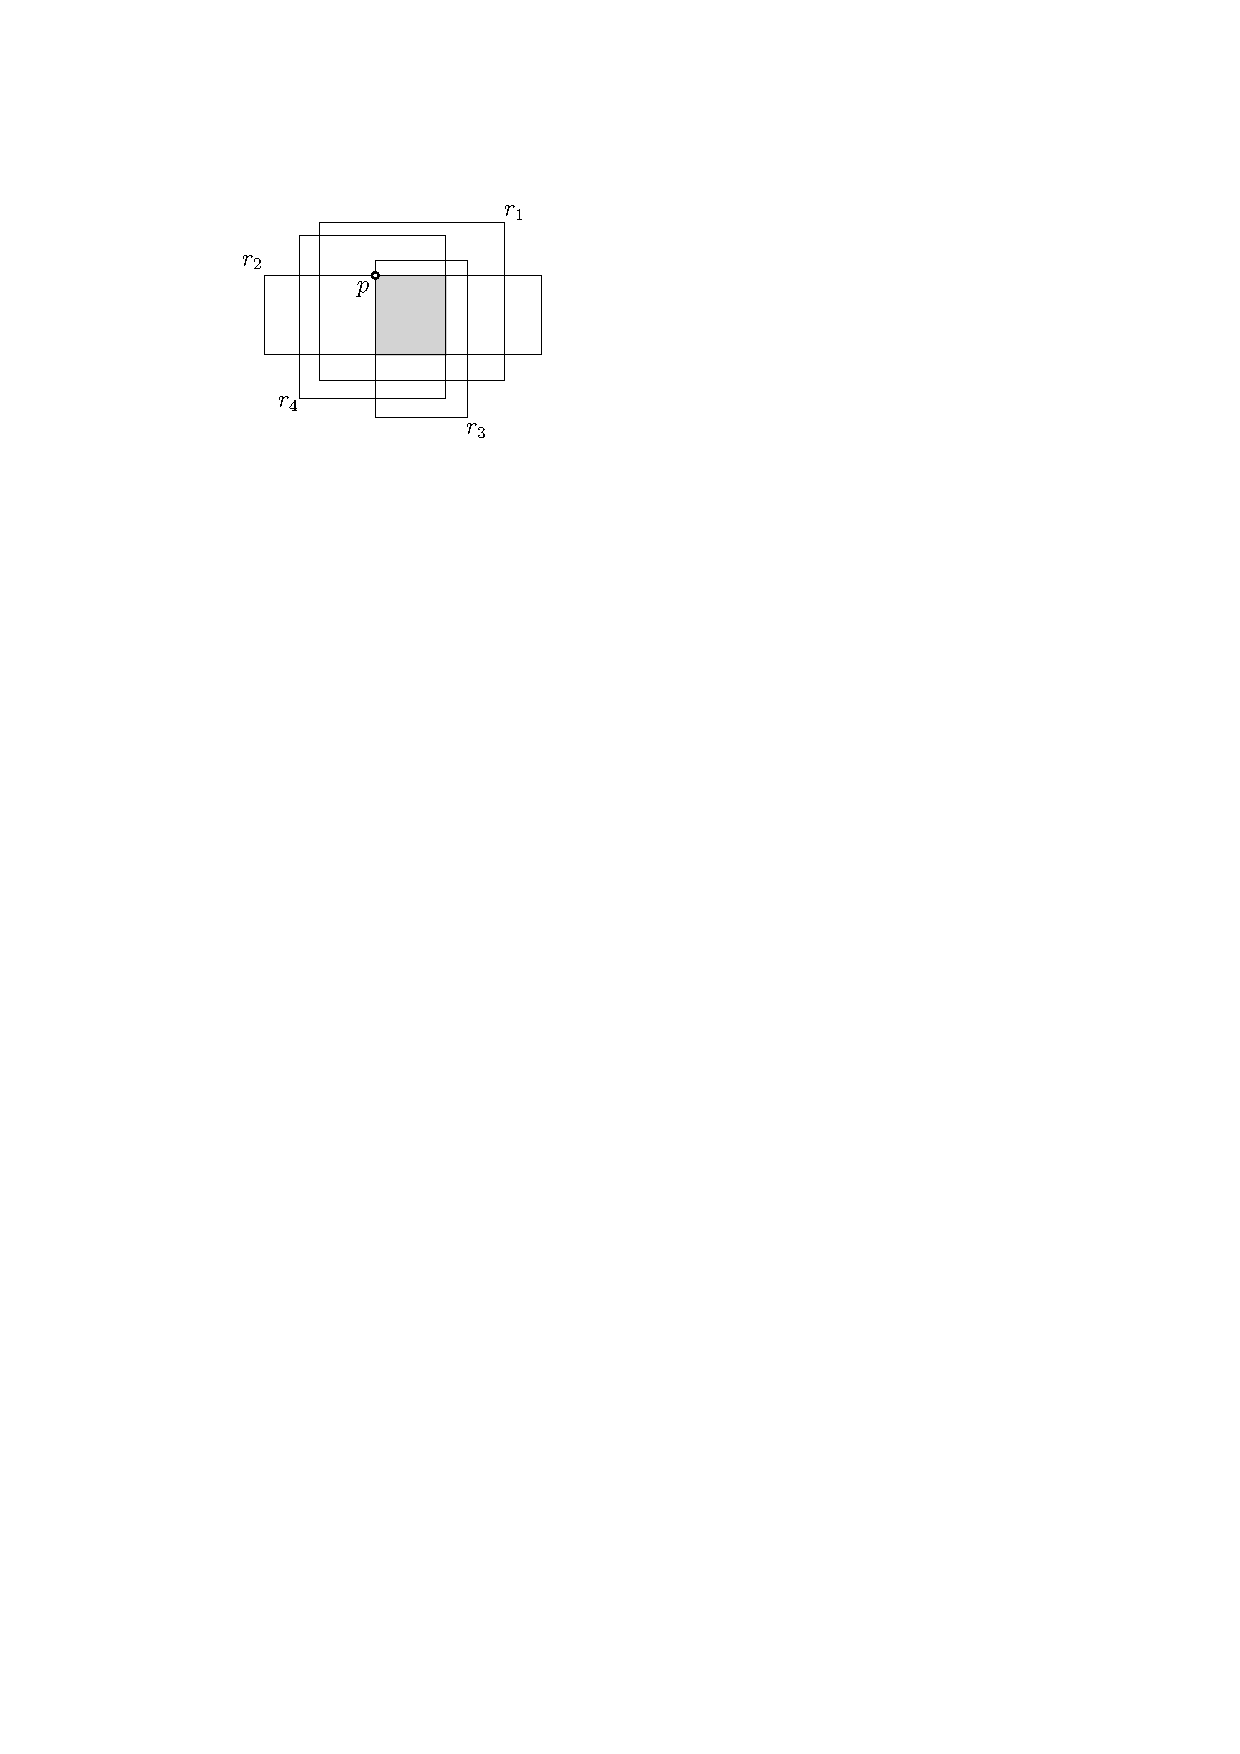
\includegraphics[height=27mm]{./artwork/cat2} \\
        (a) Category 1 &
        (b) Category 2
    \end{tabular}

    \figcapup
    \caption{Classifying $k$-SJ result tuples ($k$ = 4)}
    \label{fig:ksj:cats}
    \figcapdown
\end{figure}

\section{Settling $k$-SJ} \label{sec:ksj}

This section will tackle the $k$-SJ problem in its general form, where the input comprises $k$ sets of rectangles $R_1, R_2, ..., R_k$. The join result $\J(R_1, R_2, ..., R_k)$ is the set of $k$-tuples $\bm{t} = (r_1, r_2, ..., r_k) \in R_1 \times R_2 \times ... \times R_k$ satisfying the condition that $B_\bm{t}$ --- which is $\bigcap_{i=1}^k r_i \ne \emptyset$ (see \eqref{eqn:B_t}) --- is non-empty. 

\vgap 

Consider any result tuple $\bm{t} = (r_1, r_2, ..., r_k) \in \J(R_1, R_2, ..., R_k)$, and let $p$ be the top-left corner of $B_\bm{t}$. Depending on how $p$ is determined, we classify $\bm{t}$ into one of the two categories below: 
\myitems{
    \item {{\bf Cat.\ 1:}} $p$ is the top-left corner of $r_i$ for some $i \in [k]$. 
    
    \item {{\bf Cat.\ 2:}} $p$ is not a corner of any of $r_1, ..., r_k$. This means $p$ must be the intersection point between the top edge of some rectangle $r_i$ and the left edge of another rectangle $r_j$, where $i, j \in [k]$ and $i \ne j$.
}
Figure~\ref{fig:ksj:cats} illustrates a tuple of each category, assuming $k=4$. 

\vgap 

As stated in Theorem~\ref{thm:main-recur}, we are given an algorithm $\A$ that can solve any $(k-1)$-SJ problem in $F_{k-1}(n, \out)$ time, where $n$ and $\out$ are the input and output sizes, respectively. Equipped with $\A$, we will show how to find the result tuples of each category within the time complexity of \eqref{eqn:main:reccurrence}.

\extraspacing {\bf Category 1.} Given an $i \in [k]$, we denote by $\J^\cat_i$ the set of $k$-tuples $\bm{t} = (r_1, ..., r_k) \in \J(R_1, ..., R_k)$ such that the top-left corner of $B_\bm{t}$ is the top-left corner of $\bm{t}[i]$. We will compute $\J^\cat_i$ for $i = k$; the set $\J^\cat_i$ of every other $i$ can be produced in the same manner. 

\vgap 

For every $\bm{t} = (r_1, r_2, ..., r_k) \in \J^\cat_k$, the top-left corner of $r_k$ must be covered by all of $r_1, ..., r_{k-1}$. This observation motivates us to find $\J^\cat_i$ as follows. First, collect the set $P$ of top-left corners of all the rectangles in $R_k$. Remove from $P$ every point $p$ with the property that, there exists at least one $j \in [k-1]$ such that $p$ is covered by no rectangle in $R_j$. This requires solving $k-1$ instances of the detection version of Problem $\mathscr{A}$ (in each instance, the input includes $P$ together with a different $R_j$, $j \in [k-1]$); the cost is $O(k n \log n)$ by the discussion in Section~\ref{sec:bricks}.

\vgap 

Let $P'$ be the set of remaining points in $P$ after the aforementioned removal. Next, for each $j \in [k-1]$, solve the reporting version of Problem $\mathscr{A}$ by feeding $P'$ and $R_j$ as the input. Doing so produces, for each point $p \in P'$, the set $\contained_{R_j}(p)$, which --- as defined in \eqref{eqn:contained},  noticing that $p$ is a degenerated ``horizontal segment'' --- is the set of rectangles in $R_j$ covering $p$. By the discussion in Section~\ref{sec:bricks}, the total cost of this step is bounded by
\myeqn{
    O\Big(kn \log n + \sum_{p \in P'} \sum_{j \in [k-1]} |\contained_{R_j}(p)| \Big). \label{eqn:ksj:cat1:help1}
}

We are ready to generate $\J^\cat_k$. Take any point $p \in P'$, let $r \in R_k$ be the rectangle with $p$ as the top-left corner. For every $(k-1)$-tuple 
\myeqn{
    (r_1, ..., r_{k-1}) \in \contained_{R_1}(p) \times ... \times \contained_{R_{k-1}}(p) \label{eqn:ksj:cat1:help2}
}
we add $(r_1, ..., r_{k-1}, r)$ to $\J^\cat_k$. Performing the above for all $p \in P'$ generates the whole $\J^\cat_k$ in $O(1 + |\J^\cat_k|)$ time. The way $P'$ is computed ensures that $\contained_{R_j}(p) \ne \emptyset$ for all $j \in [k-1]$. Hence, we have $\sum_{j \in [k-1]} |\contained_{R_j}(p)| \le \prod_{j \in [k-1]} |\contained_{R_j}(p)|$, which implies that \eqref{eqn:ksj:cat1:help1} is bounded by $O(kn \log n + k \cdot |\J^\cat_k|) = O(kn \log n + k \cdot \out)$ .

\vgap 

Therefore, the total time of computing all of $\J^\cat_1, ..., \J^\cat_k$ is $O(k) \cdot (kn \log n + k \cdot \out)$. A category-1 result tuple $\bm{t}$ may be seen more than once (this happens if the top-left corner of $B_\bm{t}$ is the top-left corner of more than one rectangle in $\bm{t}$). Duplicate removal can be achieved at no extra cost asymptotically, following the ideas explained in Section~\ref{sec:hv:type2}.

\extraspacing {\bf Category 2.} Given $i, j \in [k]$ with $i \ne j$, we denote by $\J^\catt_{i,j}$ the set of $k$-tuples $\bm{t} = (r_1, ..., r_k) \in \J(R_1, ..., R_k)$ such that the top-left corner of $B_\bm{t}$ is the intersection between the top edge of $r_i$ and the left edge of $r_j$. The Category 2 of result tuples is the union of the $\J^\catt_{i,j}$ of all possible $i, j$. 

\vgap 

The computation of $\J^\catt_{i,j}$ is an instance of H-V $k$-SJ. Specifically, collect the top-edges of all rectangles $r_i \in R_i$ into a set $H$, and collect the left-edges of all rectangles $r_j \in R_j$ into a set $V$. This yields an H-V $k$-SJ problem whose input comprises all the $R_z$ with $z \in [k] \setminus \set{i,j}$,  $H$, and $V$. Its output includes every $r_z \in R_z$, for $z \in [k] \setminus \set{i,j}$, $h \in H$, and $v \in V$ such that $h \cap v \cap \bigcap_{z \in [k] \setminus \set{i,j}} r_z \ne \emptyset$. There is one-one correspondence between the output of the H-V $k$-SJ and $\J^\catt_{i,j}$. Thus, by Lemma~\ref{lmm:hv}, the H-V $k$-SJ can be solved in $O(k) \cdot (F_{k-1}(n, |\J^\catt_{i,j}|) + n \log n + k \cdot |\J^\catt_{i,j}|)$ time. Converting the output into $\J^\catt_{i,j}$ takes another $O(|\J^\catt_{i,j}|)$ time. Applying the trivial bound $|\J^\catt_{i,j}| \le \out$, we can assert that $\J^\catt_{i,j}$ can be produced in $O(k) \cdot (F_{k-1}(n, \out) + n \log n + k \cdot \out)$ time

\vgap 

Performing the above for all $i, j \in [k]$ with $i \ne j$ results in a total time complexity of $O(k^3) \cdot (F_{k-1}(n, \out) + n \log n + k \cdot \out)$. A category-1 result tuple $\bm{t}$ may be seen more than once (this happens if the top-left corner of $B_\bm{t}$ is the top-left corner of more than one rectangle in $\bm{t}$). Duplicate removal can be achieved at no extra cost asymptotically, following the ideas explained in Section~\ref{sec:hv:type2}.


\bibliographystyle{plainurl}% the mandatory bibstyle
\bibliography{ref}

\balance

\appendix 

\section*{Appendix}

\section{Building Brick Algorithms} \label{app:bricks}

\extraspacing {\bf Algorithm for Problem $\bm{\mathscr{A}}$.}

\extraspacing {\bf Algorithm for Problem $\bm{\mathscr{B}}$.}

\extraspacing {\bf Algorithm for Problem $\bm{\mathscr{C}}$.}

\extraspacing {\bf Algorithm for Problem $\bm{\mathscr{D}}$.}

\extraspacing {\bf Algorithm for Problem $\bm{\mathscr{E}}$.}


\section{Completing the Proof of Lemma~\ref{lmm:hv}} \label{app:hv} 

\extraspacing {\bf Proof of Lemma~\ref{lmm:hv:type1:recur-output}.}

\extraspacing {\bf Proof of Lemma~\ref{lmm:hv:type1:properties}.}

\extraspacing {\bf Computing $\bm{R^*_1, R^*_2, ..., R^*_{k-2}}$.}

\extraspacing {\bf Proof of Lemma~\ref{lmm:hv:type1:cross-r*}.}

\extraspacing {\bf Proof of Lemma~\ref{lmm:hv:type2:recur-output}.}

\extraspacing {\bf Proof of Lemma~\ref{lmm:hv:type2:properties}.}

\extraspacing {\bf Computing $\bm{H^*}$.}

\extraspacing {\bf Proof of Lemma~\ref{lmm:hv:type2:contained-h*}.}

\section{Hardness of 3-SJ in 3D Space} \label{app:lb-cond}

%\end{sloppy}
\end{document}

